% In this work, we adopt a customized version of the YOLO detection framework by integrating the MobileNetV4 backbone in order to obtain a lightweight yet effective object detection model. The primary motivation behind this design choice is to reduce computational complexity and memory consumption while maintaining reliable detection accuracy. Such requirements are essential for deployment on resource constrained edge devices, including embedded systems, single board computers, and mobile platforms.

% MobileNetV4 is a recently proposed convolutional neural network architecture designed for universal deployment across mobile and edge hardware. It emphasizes efficient feature extraction through improved depthwise separable convolutions, universal inverted bottleneck blocks, and optimized layer scaling strategies. Compared to conventional backbones such as CSPDarknet or standard ResNet variants, MobileNetV4 provides a more balanced trade off between inference speed and representational capability. As a result, it is particularly suitable for real time computer vision tasks where latency, power consumption, and memory footprint are critical constraints.

% \subsection{Backbone Replacement Strategy}

% To integrate MobileNetV4 into the YOLO framework, the default backbone definition is replaced by a customized model configuration file, denoted as \texttt{yolo11-mobilenetv4.yaml}. This configuration follows the standard Ultralytics YOLO model definition format while modifying the backbone section to incorporate MobileNetV4 building blocks. The neck and detection head structures remain largely unchanged in order to preserve compatibility with existing loss functions, anchor settings, and training pipelines.

% The backbone replacement process is performed at the model configuration and module registration level rather than modifying the core training logic. This design choice improves maintainability and simplifies future updates of the YOLO framework. The integration procedure follows a publicly available technical guide that details how MobileNetV4 modules are registered, parsed, and treated as backbone components during model construction\footnote{Guideline for integrating MobileNetV4 into YOLO architectures is available at \url{https://blog.csdn.net/qq_44231797/article/details/147483132}.}. By preserving the feature pyramid structure, multi scale detection capability is maintained despite the lightweight backbone.

% \subsection{Model Initialization and Pretrained Weights}

% To accelerate convergence and improve training stability, the model is initialized using pretrained weights from a lightweight YOLO variant. Specifically, the \texttt{yolo11n.pt} checkpoint is loaded as the initial parameter set. Although the backbone architecture differs from the original YOLO design, partial weight transfer remains beneficial for shared components such as the detection head and certain convolutional layers.

% The Ultralytics YOLO API automatically performs parameter matching where possible and ignores incompatible layers. This mechanism enables the model to leverage prior knowledge while avoiding structural conflicts during initialization. As a result, the training process converges more reliably compared to training from scratch.

% \subsection{Training Configuration}

% The training process is conducted using the Ultralytics YOLO training interface, which provides a flexible and reproducible pipeline for object detection tasks. Dataset information is specified through a YAML configuration file that defines training and validation paths, class labels, and metadata. All input images are resized to a resolution of $320 \times 320$ pixels in order to balance detection accuracy and computational efficiency.

% Stochastic Gradient Descent is selected as the optimization algorithm due to its stable convergence behavior for large scale detection models. Automatic mixed precision is enabled to reduce GPU memory usage and accelerate training while maintaining numerical stability. The model is trained for a total of 400 epochs to ensure sufficient convergence given the modified backbone structure.

% \subsection{Training Script}

% The complete training script used in this study is shown below. This script defines the model configuration, loads pretrained weights, and executes the training process with the selected hyperparameters.

% \begin{lstlisting}[language=Python, caption={YOLO-MobileNetV4 Training Script}]
% # Model configuration file
% model_yaml_path = r"yolo11-mobilenetv4.yaml"

% # Dataset configuration file
% data_yaml_path = r"dataset/data.yaml"

% # Pretrained model
% pre_model_name = "yolo11n.pt"

% import warnings
% warnings.filterwarnings("ignore")

% from ultralytics import YOLO

% if __name__ == "__main__":
%     model = YOLO(model_yaml_path)
%     model.load(pre_model_name)

%     model.train(
%         data=data_yaml_path,
%         cache=False,
%         imgsz=320,
%         epochs=400,
%         workers=8,
%         device="0",
%         optimizer="SGD",
%         amp=True,
%         project="runs/train-yolo-mobilenetv4",
%         name="exp"
%     )
% \end{lstlisting}

\section{YOLO-MobileNetV4 Model}

In this work, we adopt a customized version of the YOLOv26 detection framework by integrating the MobileNetV4 backbone in order to obtain a lightweight yet effective object detection model. The primary motivation behind this design choice is to reduce computational complexity and memory consumption while maintaining reliable detection accuracy. Such requirements are essential for deployment on resource constrained edge devices, including embedded systems, single board computers, and mobile platforms.

\subsection{Integrating MobileNetv4 into YOLO}

Following the our paper in \hyperref[chap:append]{Appendix}, we will continue to integrate MobileNetV4 as the feature extractor for YOLO26 creates a hybrid "YOLO-MNv4" architecture that is theoretically optimal for autonomous driving. On mobile accelerators like the Pixel EdgeTPU, MNv4 is approximately twice as fast as MobileNetV3 for equivalent accuracy due to its high operational intensity. Replacing the standard YOLO26 backbone with MNv4 significantly reduces the floating-point operations (FLOPs) required per inference. This architecture specifically excels in occlusion handling, where the advanced receptive fields of the UIB blocks allow the model to infer the presence of a traffic light even when it is partially obscured by large vehicles, ensuring a robust and reliable perception system.

To adapt the original YOLO26 architecture for edge deployment, several crucial modifications were made (comparing Figure \ref{fig:yolo26_original_arch} to Figure \ref{fig:yolo26_mnv4_arch}). First, the standard heavy CNN backbone was replaced entirely with {MobileNetV4ConvSmall050}. Second, the original 4-head Feature Pyramid Network (P2, P3, P4, P5) was scaled down to a {3-head architecture} (P3, P4, P5) by removing the high-resolution P2 feature extraction path and its corresponding detection head. This reduction dramatically lowers the computational complexity (GFLOPs) and parameter count. Meanwhile, the advanced components of the YOLO26 neck—including the {C3k2} fusion blocks, {SPPF}, {C2PSA} spatial attention, and the {One-to-One Head}-were preserved to maintain state-of-the-art detection logic.

\begin{figure}[htbp]
    \centering
    \resizebox{\textwidth}{!}{
    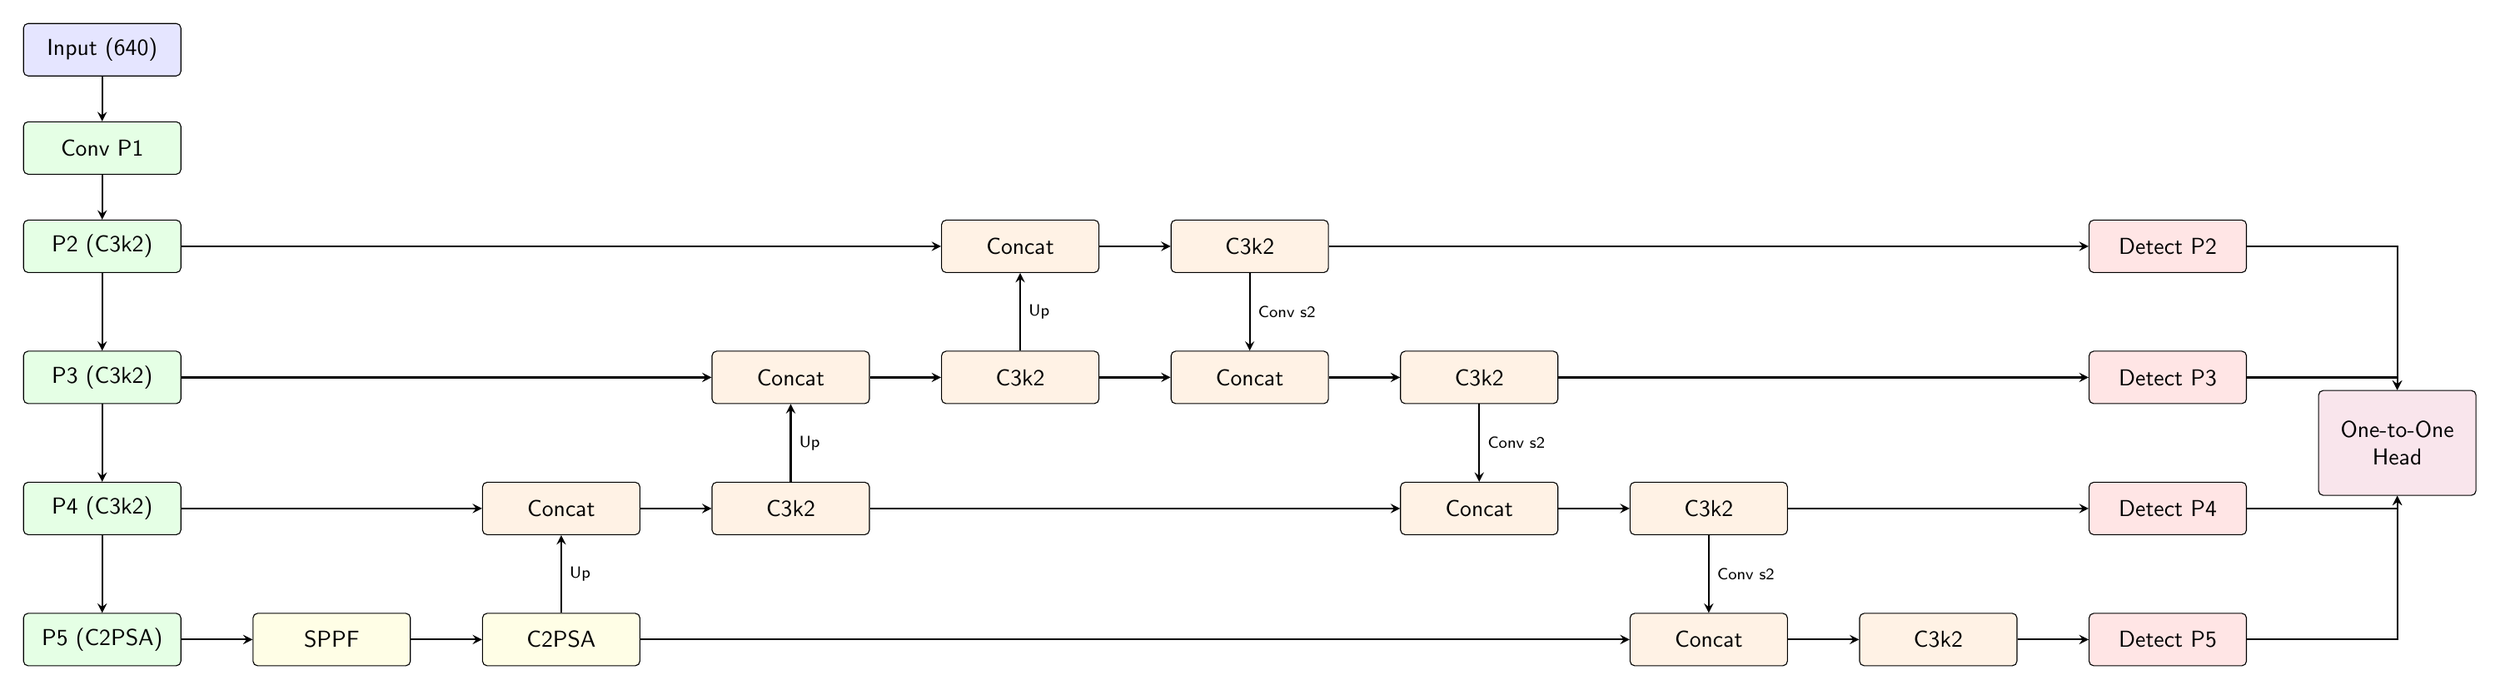
\begin{tikzpicture}[
        box/.style={rectangle, draw, minimum width=2.4cm, minimum height=0.8cm, text centered, font=\sffamily, rounded corners=2pt},
        arrow/.style={->, >=stealth, thick},
        label/.style={font=\sffamily\scriptsize}
    ]

    % Backbone
    \node[box, fill=blue!10] (input) at (0, 9) {Input (640)};
    \node[box, fill=green!10] (conv1) at (0, 7.5) {Conv P1};
    \node[box, fill=green!10] (p2) at (0, 6) {P2 (C3k2)};
    \node[box, fill=green!10] (p3) at (0, 4) {P3 (C3k2)};
    \node[box, fill=green!10] (p4) at (0, 2) {P4 (C3k2)};
    \node[box, fill=green!10] (p5) at (0, 0) {P5 (C2PSA)};

    \draw[arrow] (input) -- (conv1);
    \draw[arrow] (conv1) -- (p2);
    \draw[arrow] (p2) -- (p3);
    \draw[arrow] (p3) -- (p4);
    \draw[arrow] (p4) -- (p5);

    % SPPF & C2PSA
    \node[box, fill=yellow!10] (sppf) at (3.5, 0) {SPPF};
    \node[box, fill=yellow!10] (c2psa) at (7.0, 0) {C2PSA};
    \draw[arrow] (p5) -- (sppf);
    \draw[arrow] (sppf) -- (c2psa);

    % Neck - Top-down
    \node[box, fill=orange!10] (cat_p4) at (7.0, 2) {Concat};
    \node[box, fill=orange!10] (c3k2_td_p4) at (10.5, 2) {C3k2};
    \draw[arrow] (c2psa) -- node[right, label] {Up} (cat_p4);
    \draw[arrow] (p4) -- (cat_p4);
    \draw[arrow] (cat_p4) -- (c3k2_td_p4);

    \node[box, fill=orange!10] (cat_p3) at (10.5, 4) {Concat};
    \node[box, fill=orange!10] (c3k2_td_p3) at (14.0, 4) {C3k2};
    \draw[arrow] (c3k2_td_p4) -- node[right, label] {Up} (cat_p3);
    \draw[arrow] (p3) -- (cat_p3);
    \draw[arrow] (cat_p3) -- (c3k2_td_p3);

    \node[box, fill=orange!10] (cat_p2) at (14.0, 6) {Concat};
    \node[box, fill=orange!10] (c3k2_td_p2) at (17.5, 6) {C3k2};
    \draw[arrow] (c3k2_td_p3) -- node[right, label] {Up} (cat_p2);
    \draw[arrow] (p2) -- (cat_p2);
    \draw[arrow] (cat_p2) -- (c3k2_td_p2);

    % Neck - Bottom-up
    \node[box, fill=orange!10] (cat_p3_bu) at (17.5, 4) {Concat};
    \node[box, fill=orange!10] (c3k2_bu_p3) at (21.0, 4) {C3k2};
    \draw[arrow] (c3k2_td_p2) -- node[right, label] {Conv s2} (cat_p3_bu);
    \draw[arrow] (c3k2_td_p3) -- (cat_p3_bu);
    \draw[arrow] (cat_p3_bu) -- (c3k2_bu_p3);

    \node[box, fill=orange!10] (cat_p4_bu) at (21.0, 2) {Concat};
    \node[box, fill=orange!10] (c3k2_bu_p4) at (24.5, 2) {C3k2};
    \draw[arrow] (c3k2_bu_p3) -- node[right, label] {Conv s2} (cat_p4_bu);
    \draw[arrow] (c3k2_td_p4) -- (cat_p4_bu);
    \draw[arrow] (cat_p4_bu) -- (c3k2_bu_p4);

    \node[box, fill=orange!10] (cat_p5_bu) at (24.5, 0) {Concat};
    \node[box, fill=orange!10] (c3k2_bu_p5) at (28.0, 0) {C3k2};
    \draw[arrow] (c3k2_bu_p4) -- node[right, label] {Conv s2} (cat_p5_bu);
    \draw[arrow] (c2psa) -- (cat_p5_bu);
    \draw[arrow] (cat_p5_bu) -- (c3k2_bu_p5);

    % Detectors
    \node[box, fill=red!10] (head2) at (31.5, 6) {Detect P2};
    \node[box, fill=red!10] (head3) at (31.5, 4) {Detect P3};
    \node[box, fill=red!10] (head4) at (31.5, 2) {Detect P4};
    \node[box, fill=red!10] (head5) at (31.5, 0) {Detect P5};
    
    \node[box, fill=purple!10, align=center, minimum height=1.6cm] (detect) at (35.0, 3) {One-to-One\\Head};

    \draw[arrow] (c3k2_td_p2) -- (head2);
    \draw[arrow] (c3k2_bu_p3) -- (head3);
    \draw[arrow] (c3k2_bu_p4) -- (head4);
    \draw[arrow] (c3k2_bu_p5) -- (head5);
    
    \draw[arrow] (head2) -| (detect);
    \draw[arrow] (head3) -| (detect);
    \draw[arrow] (head4) -| (detect);
    \draw[arrow] (head5) -| (detect);

    \end{tikzpicture}
    }
    \vspace{0.5cm}
    \caption{Architecture of the original YOLO26-p2 model with 4-head detection mechanism (P2/P3/P4/P5 outputs) for standard object detection tasks. Channel widths scale with the chosen model variant (n/s/m/l/x).}
    \label{fig:yolo26_original_arch}
\end{figure}

\begin{figure}[htbp]
    \centering
    \resizebox{\textwidth}{!}{
    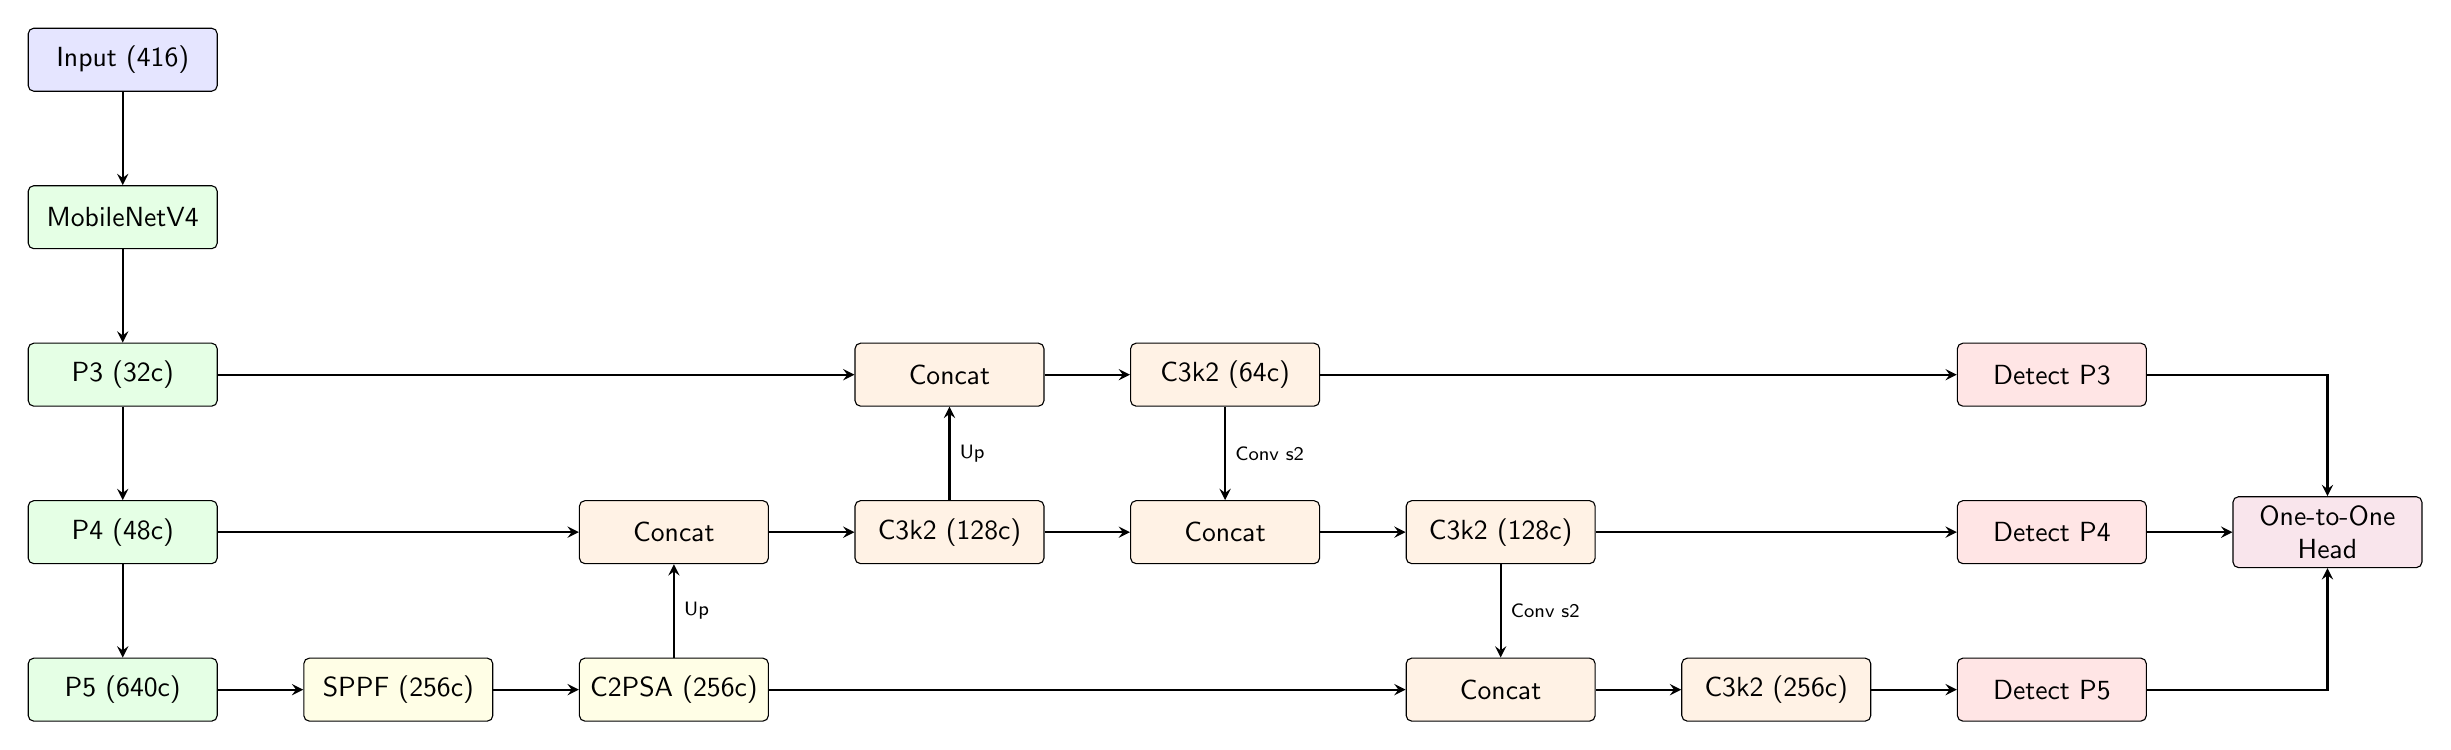
\begin{tikzpicture}[
        box/.style={rectangle, draw, minimum width=2.4cm, minimum height=0.8cm, text centered, font=\sffamily, rounded corners=2pt},
        arrow/.style={->, >=stealth, thick},
        label/.style={font=\sffamily\scriptsize}
    ]

    % X coordinates:
    % 0.0: Backbone
    % 3.5: SPPF
    % 7.0: C2PSA, cat1
    % 10.5: c3k2_1, cat2
    % 14.0: c3k2_2, cat3
    % 17.5: c3k2_3, cat4
    % 21.0: c3k2_4
    % 24.5: Detectors
    % 28.0: Head

    % Backbone
    \node[box, fill=blue!10] (input) at (0, 8) {Input (416)};
    \node[box, fill=green!10] (mnv4) at (0, 6) {MobileNetV4};
    \node[box, fill=green!10] (p3) at (0, 4) {P3 (32c)};
    \node[box, fill=green!10] (p4) at (0, 2) {P4 (48c)};
    \node[box, fill=green!10] (p5) at (0, 0) {P5 (640c)};

    \draw[arrow] (input) -- (mnv4);
    \draw[arrow] (mnv4) -- (p3);
    \draw[arrow] (p3) -- (p4);
    \draw[arrow] (p4) -- (p5);

    % SPPF & C2PSA
    \node[box, fill=yellow!10] (sppf) at (3.5, 0) {SPPF (256c)};
    \node[box, fill=yellow!10] (c2psa) at (7.0, 0) {C2PSA (256c)};
    \draw[arrow] (p5) -- (sppf);
    \draw[arrow] (sppf) -- (c2psa);

    % Neck - Top-down
    \node[box, fill=orange!10] (cat1) at (7.0, 2) {Concat};
    \node[box, fill=orange!10] (c3k2_1) at (10.5, 2) {C3k2 (128c)};
    \draw[arrow] (c2psa) -- node[right, label] {Up} (cat1);
    \draw[arrow] (p4) -- (cat1);
    \draw[arrow] (cat1) -- (c3k2_1);

    \node[box, fill=orange!10] (cat2) at (10.5, 4) {Concat};
    \node[box, fill=orange!10] (c3k2_2) at (14.0, 4) {C3k2 (64c)};
    \draw[arrow] (c3k2_1) -- node[right, label] {Up} (cat2);
    \draw[arrow] (p3) -- (cat2);
    \draw[arrow] (cat2) -- (c3k2_2);

    % Neck - Bottom-up
    \node[box, fill=orange!10] (cat3) at (14.0, 2) {Concat};
    \node[box, fill=orange!10] (c3k2_3) at (17.5, 2) {C3k2 (128c)};
    \draw[arrow] (c3k2_2) -- node[right, label] {Conv s2} (cat3);
    \draw[arrow] (c3k2_1) -- (cat3);
    \draw[arrow] (cat3) -- (c3k2_3);

    \node[box, fill=orange!10] (cat4) at (17.5, 0) {Concat};
    \node[box, fill=orange!10] (c3k2_4) at (21.0, 0) {C3k2 (256c)};
    \draw[arrow] (c3k2_3) -- node[right, label] {Conv s2} (cat4);
    \draw[arrow] (c2psa) -- (cat4);
    \draw[arrow] (cat4) -- (c3k2_4);

    % Detectors
    \node[box, fill=red!10] (head1) at (24.5, 4) {Detect P3};
    \node[box, fill=red!10] (head2) at (24.5, 2) {Detect P4};
    \node[box, fill=red!10] (head3) at (24.5, 0) {Detect P5};
    
    \node[box, fill=purple!10, align=center] (detect) at (28.0, 2) {One-to-One\\Head};

    \draw[arrow] (c3k2_2) -- (head1);
    \draw[arrow] (c3k2_3) -- (head2);
    \draw[arrow] (c3k2_4) -- (head3);
    
    \draw[arrow] (head1) -| (detect);
    \draw[arrow] (head2) -- (detect);
    \draw[arrow] (head3) -| (detect);

    \end{tikzpicture}
    }
    \vspace{0.5cm} % Add some space before caption to prevent overlap
    \caption{Architecture of the YOLO26 model with MobileNetV4ConvSmall050 backbone, dual-head mechanism, and NMS-free end-to-end detection, tailored for $416\times416$ resolution.}
    \label{fig:yolo26_mnv4_arch}
\end{figure}

% \subsection{Training Hyperparameters}

% The training process is conducted using the Ultralytics YOLO training API, which provides a reproducible and configurable pipeline for object detection tasks. The dataset is specified through a YAML configuration file (\texttt{TrafficLightV5.v9i.yolo26/data.yaml}) that defines training and validation image paths, class labels, and metadata. To bootstrap training, pretrained weights from \texttt{yolo26n.pt} are loaded via partial weight transfer; compatible layers (primarily in the neck and head) inherit learned parameters, while the MobileNetV4 backbone is initialised from scratch. The \texttt{end2end=True} flag activates the One-to-One head for NMS-free training. Table~\ref{tab:hyperparams} summarises the key hyperparameters.

% \begin{table}[htbp]
% \centering
% \caption{Selected training hyperparameters for the YOLO26-MobileNetV4 model.}
% \label{tab:hyperparams}
% \renewcommand{\arraystretch}{1.15}
% \begin{tabular}{l l l}
% \hline
% \textbf{Parameter} & \textbf{Value} & \textbf{Rationale} \\
% \hline
% \texttt{imgsz} & $416 \times 416$ & Balance between spatial resolution and edge inference speed \\
% \texttt{epochs} & 100 & Sufficient convergence for the modified backbone \\
% \texttt{batch} & 16 & Fits within GPU memory with MobileNetV4 backbone \\
% \texttt{patience} & 100 & Disable early stopping; run full cosine LR cycle \\
% \texttt{optimizer} & auto (SGD) & Stable convergence for detection models \\
% \texttt{lr0} & 0.005 & Slightly elevated initial LR for unfrozen backbone \\
% \texttt{lrf} & 0.01 & Final LR ratio: $\text{lr}_{\text{final}} = 0.01 \times \text{lr}_0$ \\
% \texttt{cos\_lr} & True & Cosine annealing for smooth convergence in late epochs \\
% \texttt{warmup\_epochs} & 3.0 & Gradual LR ramp-up to stabilise early gradients \\
% \texttt{amp} & True & Mixed-precision training for memory efficiency \\
% \texttt{freeze} & None & All layers trainable; no backbone freezing \\
% \texttt{close\_mosaic} & 10 & Disable mosaic augmentation in the last 10 epochs \\
% \hline
% \texttt{box} & 7.5 & Bounding box regression loss weight \\
% \texttt{cls} & 0.5 & Classification loss weight \\
% \texttt{dfl} & 1.5 & DFL loss weight (set but unused since YOLO26 removes DFL) \\
% \hline
% \end{tabular}
% \end{table}

% \subsubsection{Optimiser and Learning Rate Schedule}
% The optimiser is set to \texttt{auto}, which defaults to Stochastic Gradient Descent (SGD) with Nesterov momentum ($\mu = 0.937$) and weight decay ($\lambda = 5 \times 10^{-4}$). The initial learning rate is set to $\text{lr}_0 = 0.005$, slightly higher than the default $0.01$ to compensate for the unfrozen MobileNetV4 backbone requiring larger gradient steps to adapt to the traffic light domain. A cosine annealing schedule (\texttt{cos\_lr=True}) smoothly decays the learning rate to $\text{lr}_0 \times \text{lrf} = 5 \times 10^{-5}$ over the full 100 epochs, ensuring fine-grained convergence in the later stages of training without the abrupt transitions of step-decay schedules.

% \subsubsection{No Backbone Freezing}
% Unlike transfer learning approaches that freeze the backbone during initial epochs, this configuration leaves all layers trainable (\texttt{freeze=None}). Since the MobileNetV4ConvSmall050 backbone differs fundamentally from the original YOLO26 backbone, the pretrained weights only partially transfer. Freezing would prevent the new backbone from learning domain-specific features such as the distinctive shapes and colours of Vietnamese traffic light signal heads and arrow indicators.

% \subsubsection{Image Augmentation Strategy}
% The augmentation pipeline is carefully tuned for the traffic light detection domain:

% \begin{itemize}
%     \item \textbf{Colour jitter}: Hue shift is minimal (\texttt{hsv\_h}$=0.015$) to preserve the critical red/green/yellow colour semantics of traffic signals. Saturation (\texttt{hsv\_s}$=0.7$) and brightness (\texttt{hsv\_v}$=0.4$) augmentation are moderate to improve robustness under varying lighting conditions without corrupting colour-dependent class distinctions.
%     \item \textbf{Geometric transforms}: Translation (\texttt{translate}$=0.1$) and scale (\texttt{scale}$=0.5$) are enabled to simulate varying camera distances and positions. Rotation (\texttt{degrees}$=0.0$) and shear (\texttt{shear}$=0.0$) are disabled since traffic lights are always vertically oriented.
%     \item \textbf{Flipping disabled}: Both horizontal (\texttt{fliplr}$=0.0$) and vertical (\texttt{flipud}$=0.0$) flips are strictly disabled. Horizontal flipping would reverse the direction of left/right arrow turn signals, creating incorrect training labels.
%     \item \textbf{Mosaic}: Set to 0.5 probability to composite multiple training images into one frame, improving the model's ability to detect small, densely packed objects such as timer digit clusters. Mosaic is automatically disabled in the last 10 epochs (\texttt{close\_mosaic}$=10$) so the model fine-tunes on unmodified real images.
%     \item \textbf{MixUp and CopyPaste}: Both disabled (\texttt{mixup}$=0.0$, \texttt{copy\_paste}$=0.0$) to avoid blending signals from different classes, which could confuse the network on colour-critical traffic light states.
% \end{itemize}


\subsection{Dataset and Hyper parameters}
\label{sub:datasetYolo}
A well-prepared dataset and carefully tuned hyperparameters are essential for successfully training the modified YOLO-MobileNetV4 model. This section details the dataset used for traffic light detection, including its composition and pre-processing steps, before explaining the specific training configurations and augmentation strategies applied to ensure robust performance.

\subsubsection{Dataset Composition and Pre-processing}
The model is trained and evaluated on the \texttt{TrafficLightV5.v9i.yolo26} dataset, which comprises a total of 4,867 images. The dataset is annotated in the YOLO format and structured to detect four classes: \texttt{left}, \texttt{right}, \texttt{straight}, and \texttt{timer}. The images are partitioned into three splits: 4,260 images for training, 406 for validation, and 201 for testing. Prior to model ingestion, offline pre-processing and augmentations were applied via Roboflow. The pre-processing includes auto-orientation and resizing to $416 \times 416$ pixels (fit with black edges). The offline augmentation strategy generates three versions of each source image by applying random rotation ($-5^\circ$ to $+5^\circ$), random shear ($-2^\circ$ to $+2^\circ$), exposure adjustments ($\pm 10\%$), and salt-and-pepper noise ($0.1\%$ of pixels).

\subsubsection{Training Configuration}
The training process is conducted using the Ultralytics YOLO training API, which provides a reproducible and configurable pipeline for object detection tasks. The dataset is specified through a YAML configuration file (\texttt{TrafficLightV5.v9i.yolo26/data.yaml}) that defines training and validation image paths, class labels, and metadata. To bootstrap training, pretrained weights from \texttt{yolo26n.pt} are loaded via partial weight transfer; compatible layers (primarily in the neck and head) inherit learned parameters, while the MobileNetV4 backbone is initialised from scratch. The \texttt{end2end=True} flag activates the One-to-One head for NMS-free training. Table~\ref{tab:hyperparams} summarises the key hyperparameters.

\begin{table}[htbp]
\centering
\caption{Selected training hyperparameters for the YOLO26-MobileNetV4 model.}
\label{tab:hyperparams}
\renewcommand{\arraystretch}{1.15}
\begin{tabular}{l l l}
\hline
\textbf{Parameter} & \textbf{Value} & \textbf{Rationale} \\
\hline
\texttt{imgsz} & $416 \times 416$ & Balance between spatial resolution and edge inference speed \\
\texttt{epochs} & 100 & Sufficient convergence for the modified backbone \\
\texttt{batch} & 16 & Fits within GPU memory with MobileNetV4 backbone \\
\texttt{patience} & 100 & Disable early stopping; run full cosine LR cycle \\
\texttt{optimizer} & auto (SGD) & Stable convergence for detection models \\
\texttt{lr0} & 0.005 & Slightly elevated initial LR for unfrozen backbone \\
\texttt{lrf} & 0.01 & Final LR ratio: $\text{lr}_{\text{final}} = 0.01 \times \text{lr}_0$ \\
\texttt{cos\_lr} & True & Cosine annealing for smooth convergence in late epochs \\
\texttt{warmup\_epochs} & 3.0 & Gradual LR ramp-up to stabilise early gradients \\
\texttt{amp} & True & Mixed-precision training for memory efficiency \\
\texttt{freeze} & None & All layers trainable; no backbone freezing \\
\texttt{close\_mosaic} & 10 & Disable mosaic augmentation in the last 10 epochs \\
\hline
\texttt{box} & 7.5 & Bounding box regression loss weight \\
\texttt{cls} & 0.5 & Classification loss weight \\
\texttt{dfl} & 1.5 & DFL loss weight (set but unused since YOLO26 removes DFL) \\
\hline
\end{tabular}
\end{table}

\subsubsection{Optimiser and Learning Rate Schedule}
The optimiser is set to \texttt{auto}, which defaults to Stochastic Gradient Descent (SGD) with Nesterov momentum ($\mu = 0.937$) and weight decay ($\lambda = 5 \times 10^{-4}$). The initial learning rate is set to $\text{lr}_0 = 0.005$, slightly higher than the default $0.01$ to compensate for the unfrozen MobileNetV4 backbone requiring larger gradient steps to adapt to the traffic light domain. A cosine annealing schedule (\texttt{cos\_lr=True}) smoothly decays the learning rate to $\text{lr}_0 \times \text{lrf} = 5 \times 10^{-5}$ over the full 100 epochs, ensuring fine-grained convergence in the later stages of training without the abrupt transitions of step-decay schedules.

\subsubsection{No Backbone Freezing}
Unlike transfer learning approaches that freeze the backbone during initial epochs, this configuration leaves all layers trainable (\texttt{freeze=None}). Since the MobileNetV4ConvSmall050 backbone differs fundamentally from the original YOLO26 backbone, the pretrained weights only partially transfer. Freezing would prevent the new backbone from learning domain-specific features such as the distinctive shapes and colours of Vietnamese traffic light signal heads and arrow indicators.

\subsubsection{Image Augmentation Strategy}
The augmentation pipeline is carefully tuned for the traffic light detection domain:

\begin{itemize}
    \item \textbf{Colour jitter}: Hue shift is minimal (\texttt{hsv\_h}$=0.015$) to preserve the critical red/green/yellow colour semantics of traffic signals. Saturation (\texttt{hsv\_s}$=0.7$) and brightness (\texttt{hsv\_v}$=0.4$) augmentation are moderate to improve robustness under varying lighting conditions without corrupting colour-dependent class distinctions.
    \item \textbf{Geometric transforms}: Translation (\texttt{translate}$=0.1$) and scale (\texttt{scale}$=0.5$) are enabled to simulate varying camera distances and positions. Rotation (\texttt{degrees}$=0.0$) and shear (\texttt{shear}$=0.0$) are disabled since traffic lights are always vertically oriented.
    \item \textbf{Flipping disabled}: Both horizontal (\texttt{fliplr}$=0.0$) and vertical (\texttt{flipud}$=0.0$) flips are strictly disabled. Horizontal flipping would reverse the direction of left/right arrow turn signals, creating incorrect training labels.
    \item \textbf{Mosaic}: Set to 0.5 probability to composite multiple training images into one frame, improving the model's ability to detect small, densely packed objects such as timer digit clusters. Mosaic is automatically disabled in the last 10 epochs (\texttt{close\_mosaic}$=10$) so the model fine-tunes on unmodified real images.
    \item \textbf{MixUp and CopyPaste}: Both disabled (\texttt{mixup}$=0.0$, \texttt{copy\_paste}$=0.0$) to avoid blending signals from different classes, which could confuse the network on colour-critical traffic light states.
\end{itemize}

\subsection{Exporting to TFLite with INT8 Quantisation}

To deploy the trained YOLO26-MobileNetV4 model on edge devices such as the Raspberry Pi 5, the model must be converted from its native PyTorch format to TensorFlow Lite (TFLite). The Ultralytics export pipeline automates this multi-stage conversion: PyTorch $\to$ ONNX $\to$ TensorFlow SavedModel $\to$ TFLite. The export is performed with the following configuration:

\begin{lstlisting}[language=Python, caption={YOLO26-MobileNetV4 TFLite export script.}, label={lst:export}]
from ultralytics import YOLO

model = YOLO("runs/train/yolo26_mobilenetv4_custom/weights/best.pt")

model.export(
    format="tflite",
    imgsz=416,
    int8=True,
    data='TrafficLightV5.v9i.yolo26/data.yaml',
    batch=1,
    end2end=True,
)
\end{lstlisting}

\subsubsection{INT8 Post-Training Quantisation.}
Full-integer quantisation maps all floating-point weights and activations to 8-bit integers, reducing the model size by approximately $4\times$ and enabling the use of integer-only arithmetic on ARM NEON SIMD units. The quantisation scheme represents each tensor value $x$ as:

\begin{equation}
\label{eq:quant}
  x_q = \text{round}\!\left(\frac{x}{s}\right) + z,
  \qquad
  s = \frac{x_{\max} - x_{\min}}{255},
  \qquad
  z = \text{round}\!\left(-\frac{x_{\min}}{s}\right),
\end{equation}

where $s$ is the per-tensor scale factor and $z$ is the zero-point, both determined during the calibration phase. To compute these statistics, a representative subset of training images from the dataset specified by the \texttt{data} parameter is fed through the network. This calibration step records the dynamic range of each activation tensor, enabling the converter to choose optimal scale and zero-point values that minimise quantisation error across the domain-specific input distribution.

\subsubsection{End-to-End Export}
The \texttt{end2end=True} flag preserves the One-to-One detection head in the exported model graph, ensuring that the TFLite model produces final detection results directly without requiring an external NMS post-processing step. This is critical for edge deployment because it eliminates the need for custom NMS operators that may not be supported by all TFLite delegates, and guarantees deterministic output tensor shapes $(1, 300, 6)$ regardless of input content.

\subsubsection{Deployment Considerations}
The resulting INT8 TFLite model is deployed via the LiteRT (formerly TensorFlow Lite) interpreter on the target device. With \texttt{batch=1} and \texttt{imgsz=416}, the model is optimised for single-frame, real-time inference. The quantised flatbuffer file is significantly smaller than the original float32 model, fitting within the L2 cache of the Cortex-A76 cores on the Raspberry Pi 5, which minimises memory access latency during inference.

% \subsubsection{Accuracy}

% Based on the quantitative trends observed in Figures~\ref{fig:yolomobilenetv4} and~\ref{fig:code_generation}, the original YOLOv11n model achieves slightly higher detection accuracy compared to the YOLOv11n-MobileNetV4 variant. Specifically, the original model attains marginally better precision, recall, and mean Average Precision across the evaluated metrics.

% From the mAP@50 curves, the original YOLOv11n model achieves an improvement of approximately 10--15\% compared to the MobileNetV4-based model. A similar performance gap is observed for mAP@50--95, where the original architecture demonstrates around 10--15\% higher accuracy under stricter localization thresholds. These differences indicate that the original backbone provides stronger feature representation capability, particularly for precise object localization.

% Nevertheless, the overall performance gap remains relatively small. The YOLO-MobileNetV4 model preserves more than 95\% of the detection accuracy achieved by the original YOLOv11n while significantly reducing model complexity. Precision and recall curves further confirm that both models exhibit comparable convergence behavior, with the MobileNetV4 variant showing slightly lower but stable accuracy throughout training.

% These results highlight a clear trade off between accuracy and efficiency. While the original YOLOv11n model offers slightly superior detection accuracy, the YOLO-MobileNetV4 configuration provides a more balanced solution by achieving competitive accuracy with reduced computational cost. This balance makes the MobileNetV4-based model particularly suitable for deployment in edge oriented and resource constrained environments where efficiency is a primary concern.


% \begin{figure}[H]
%     \centering
%     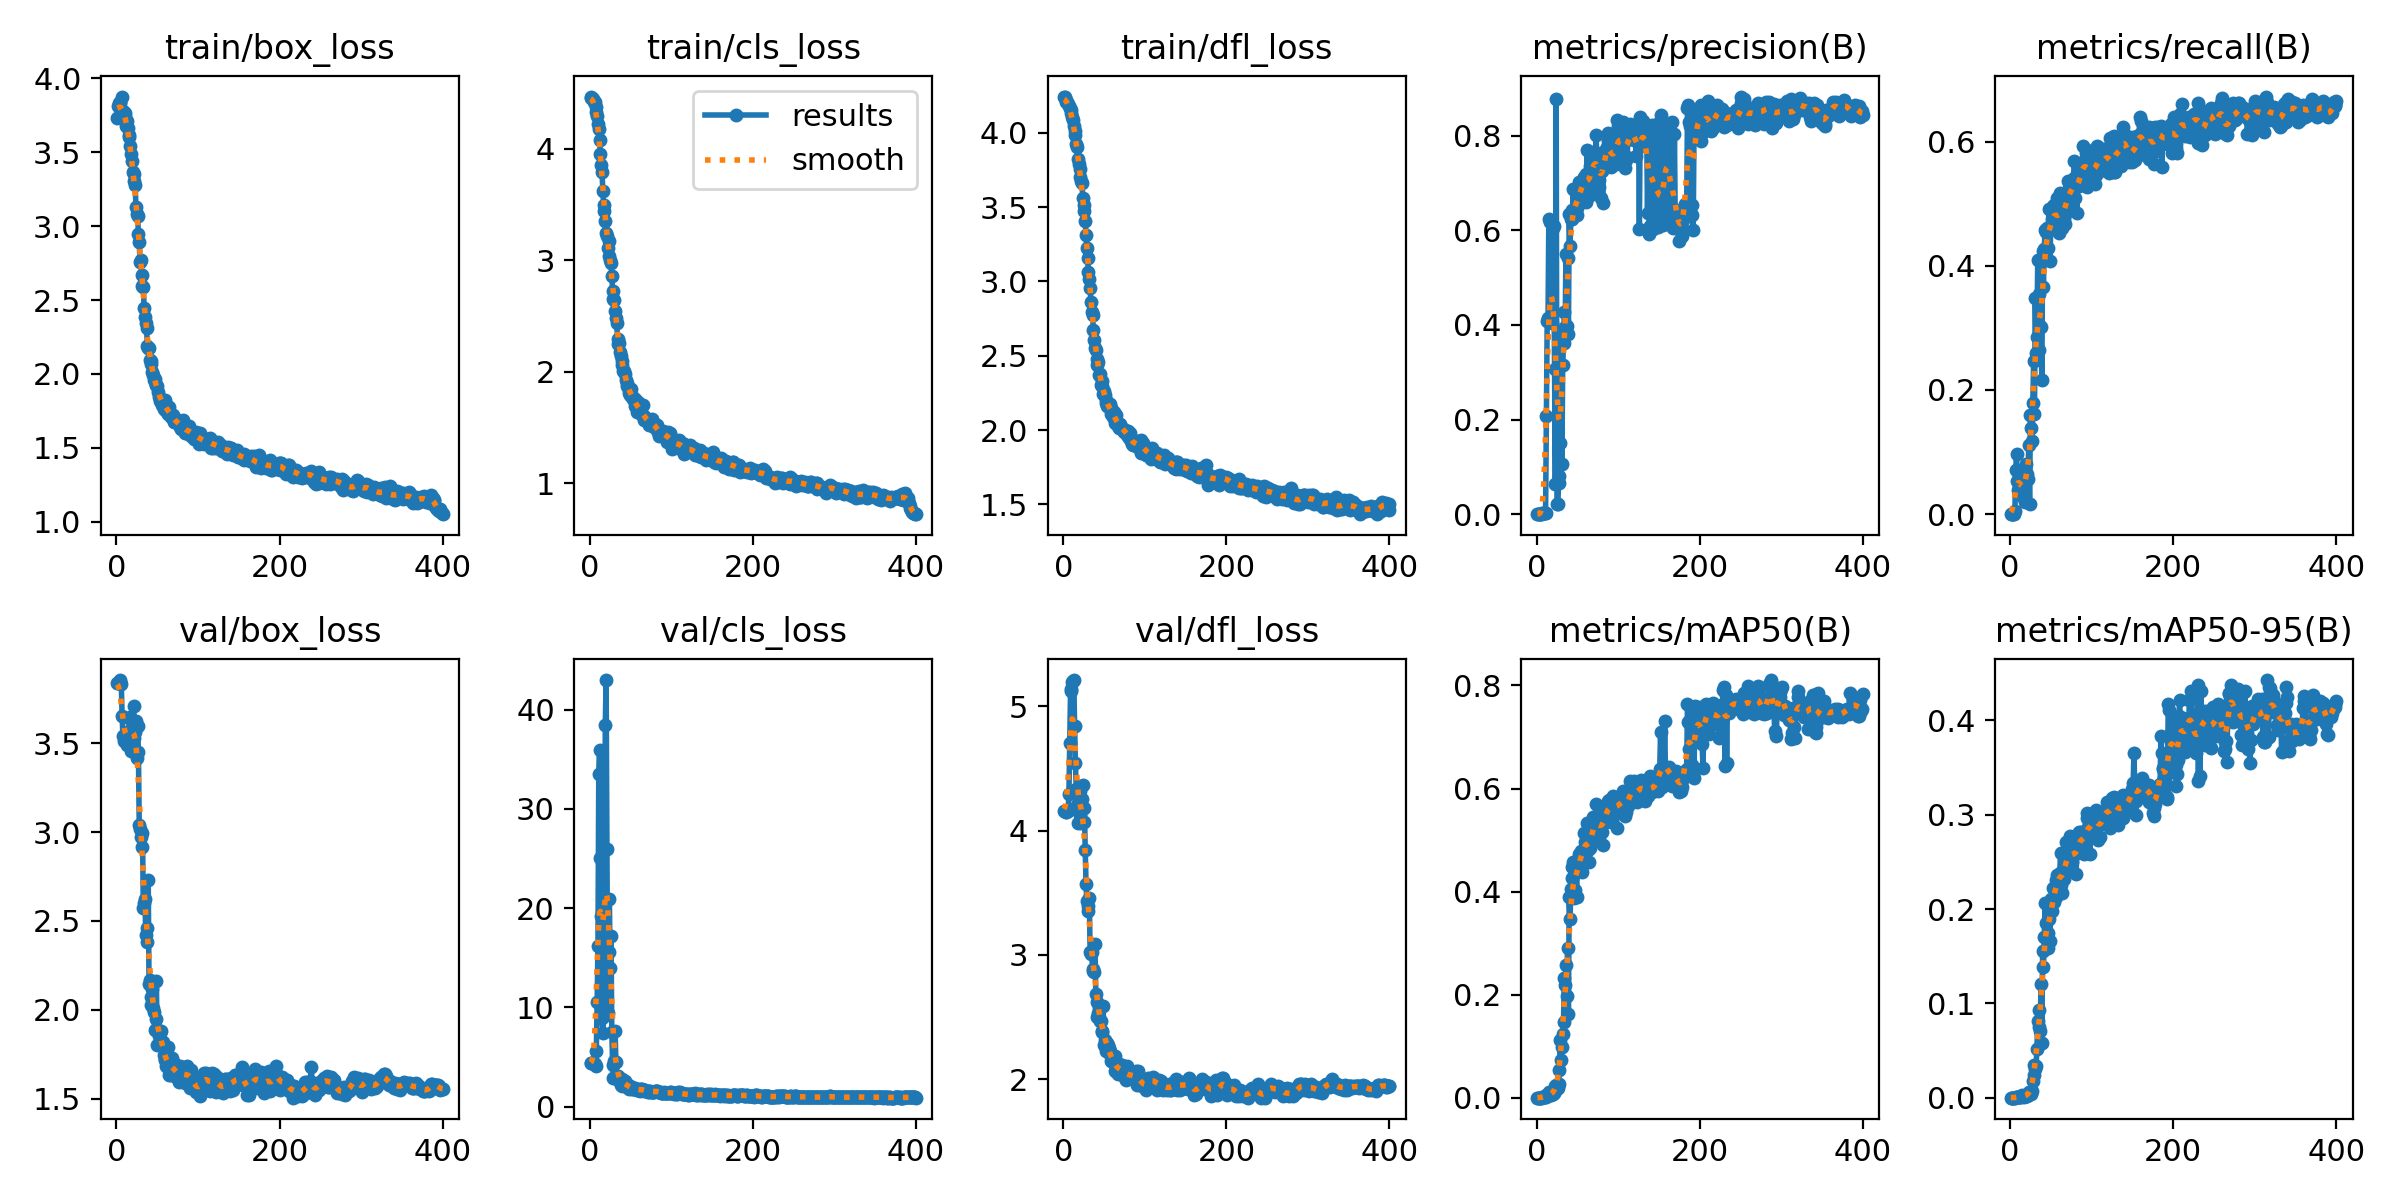
\includegraphics[width=0.75\textwidth]{Images/chap3/yolo/yolomobilenetv4.png}
%     \vspace{0.5cm}
%     \caption{The accuracy of Yolov11n-MobileNetV4}
%     \label{fig:yolomobilenetv4}
% \end{figure}

% \begin{figure}[H]
%     \centering
%     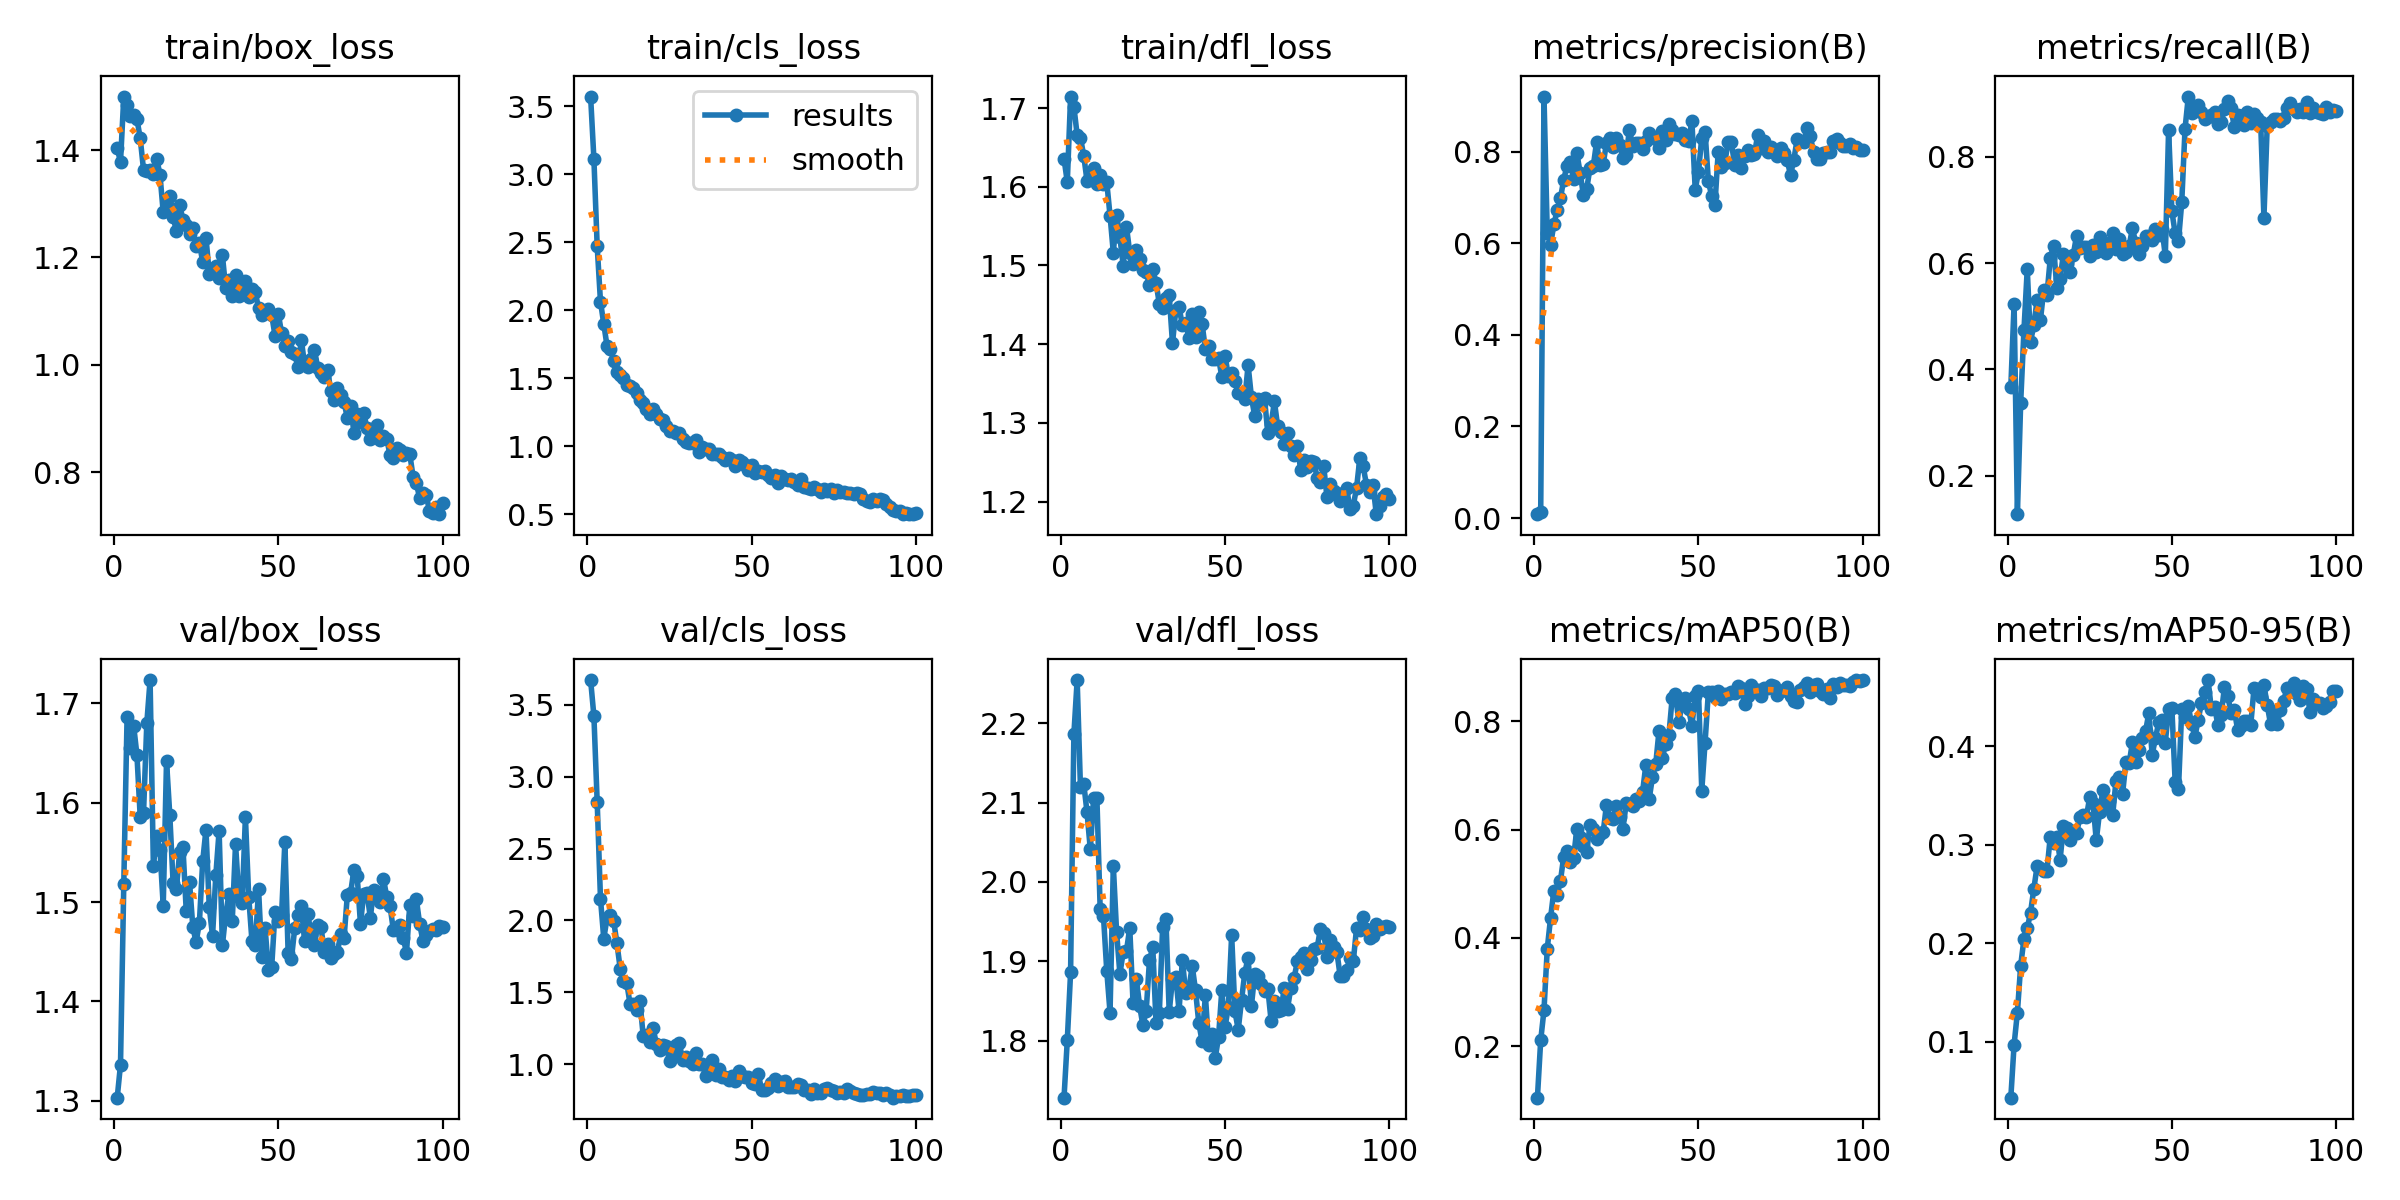
\includegraphics[width=0.75\textwidth]{Images/chap3/yolo/original.png}
%     \vspace{0.5cm}
%     \caption{The accuracy of original Yolov11n}
%     \label{fig:yolo11n}
% \end{figure}

% \subsubsection{Inference Speed}

% Inference speed is a key requirement for real time deployment on resource constrained platforms such as Raspberry Pi. According to the official Ultralytics benchmark, the original YOLO model converted to TensorFlow Lite requires more than 400\,ms per inference on Raspberry Pi class hardware when executed on CPU\footnote{Detailed benchmarking results for YOLO models on Raspberry Pi are reported by Ultralytics at \url{https://docs.ultralytics.com/vi/guides/raspberry-pi/\#detailed-comparison-table}.}. This latency corresponds to a processing rate of approximately 2--3 frames per second, which is insufficient for real time applications.

% In contrast, experimental results obtained in this work show that the YOLO-MobileNetV4 model achieves an average inference time of 30--40\,ms per frame after conversion to the TFLite format. This corresponds to an effective processing speed of approximately 25--33 frames per second. Compared to the original YOLO TFLite model, the MobileNetV4 based configuration reduces inference latency by approximately 360--370\,ms per frame.

% In relative terms, this represents a speed improvement of about 10--13 times. Equivalently, the inference time is reduced by approximately 90--92\% compared to the original YOLO TFLite implementation. Such a significant reduction enables near real time performance on CPU only embedded devices.

% The observed speedup is primarily attributed to the lightweight architecture of the MobileNetV4 backbone, which substantially reduces the number of parameters and floating point operations. As a result, the YOLO-MobileNetV4 model achieves a much more favorable balance between detection accuracy and inference speed, making it well suited for real time edge deployment on Raspberry Pi platforms.

% \begin{figure}[H]
%     \centering
%     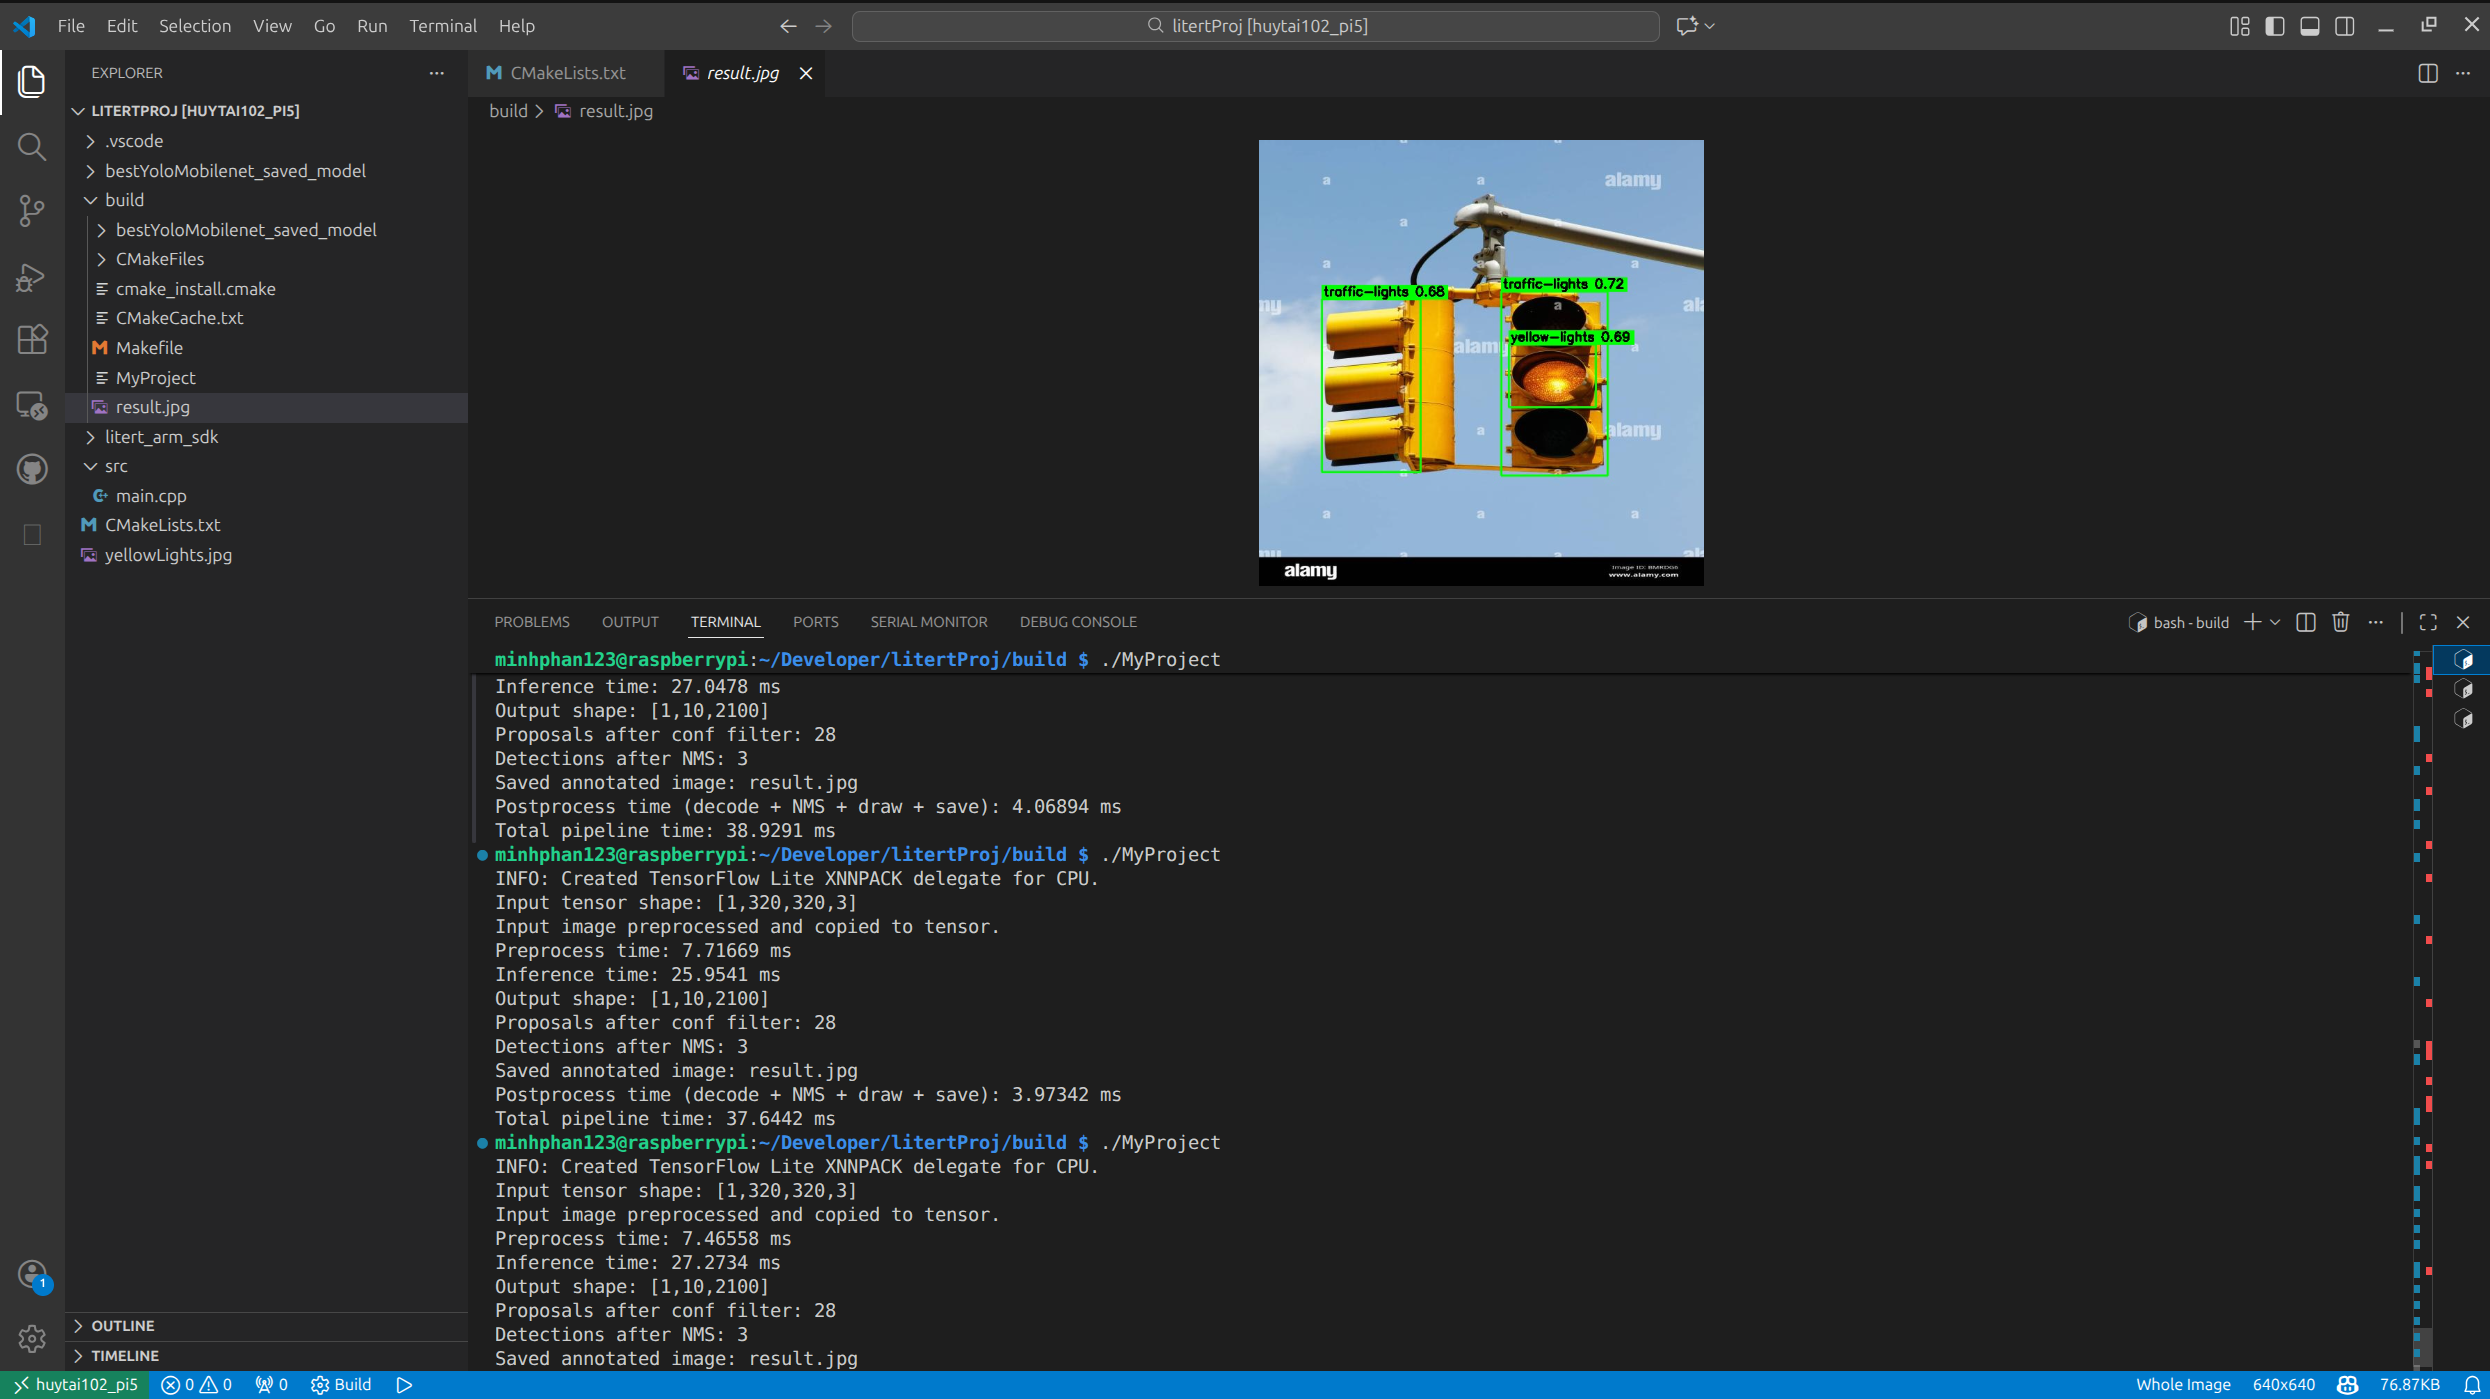
\includegraphics[width=0.75\textwidth]{Images/chap3/yolo/inference_speed.png}
%     \vspace{0.5cm}
%     \caption{The inference time of Yolovv11n-MobileNetV4 model}
%     \label{fig:infer_time_yolo11n_mobilenetv4}
% \end{figure}


% \begin{table}[H]
% \centering
% \label{tab:tradeoff_yolo_models}
% \begin{tabular}{|l|c|c|}
% \hline
% \textbf{Metric} & \textbf{YOLOv11n (Original)} & \textbf{YOLOv11n-MobileNetV4} \\
% \hline
% Backbone & CSP-based YOLO backbone & MobileNetV4 (lightweight) \\
% \hline
% mAP@50 & Higher ($\approx$ +10--15\%) & Slightly lower \\
% \hline
% mAP@50--95 & Higher ($\approx$ +10--15\%) & Slightly lower \\
% \hline
% Precision / Recall & Marginally higher & Comparable and stable \\
% \hline
% Inference time (TFLite, CPU) & $>$400 ms & 30--40 ms \\
% \hline
% Throughput (FPS) & 2--3 FPS & 25--33 FPS \\
% \hline
% Speedup factor & 1$\times$ (baseline) & $\approx$10--13$\times$ faster \\
% \hline
% Inference time reduction & -- & $\approx$90--92\% \\
% \hline
% Model complexity & Higher & Significantly reduced \\
% \hline
% Suitability for edge deployment & Limited & Highly suitable \\
% \hline
% \textbf{Overall trade-off} & Higher accuracy & Better accuracy--speed balance \\
% \hline
% \end{tabular}
% \caption{Trade-off comparison between YOLOv11n and YOLOv11n-MobileNetV4}
% \end{table}

\subsection{Evaluation between Models}

To validate the architectural modifications introduced by the MobileNetV4 backbone replacement, a systematic benchmark was conducted comparing the original YOLO26n model against the proposed YOLO26n-MobileNetV4 variant. 

Both models were evaluated on the same TrafficLightV5 validation set under identical conditions: $416 \times 416$ input resolution, INT8 TFLite quantisation, batch size of 1, and end-to-end (NMS-free) inference mode. Table~\ref{tab:model_eval} summarises the results across latency and accuracy metrics.

\begin{table}[htbp]
\centering
\caption{Performance and accuracy comparison: YOLO26n Original vs.\ YOLO26n-MobileNetV4. Negative values in the change column indicate reduction (improvement for latency metrics; degradation for accuracy metrics). Asterisks (*) denote metrics where a decrease is an expected trade-off.}
\label{tab:model_eval}
\renewcommand{\arraystretch}{1.20}
\begin{tabular}{l r r r}
\hline
\textbf{Metric} & \textbf{YOLO26n Original} & \textbf{YOLO26n-MNv4} & \textbf{Change (\%)} \\
\hline
Samples processed           & 1\,074        & \textbf{1\,366}        & $+27.19$  \\
Avg.\ latency (Pi 5)        & 55.09\,ms     & \textbf{43.23\,ms}     & $-21.52$  \\
Max spike latency (Pi 5)    & 159.73\,ms    & \textbf{78.64\,ms}     & $-50.77$  \\
Min latency (Pi 5)          & 50.12\,ms     & \textbf{36.50\,ms}     & $-27.16$  \\
CPU inference (Intel)       & 15.21\,ms     & \textbf{12.33\,ms}     & $-18.93$  \\
mAP50                       & \textbf{89.90\%}       & 85.75\%       & $-4.15$\textsuperscript{*}  \\
mAP50--95                   & \textbf{56.61\% }      & 53.31\%       & $-3.30$\textsuperscript{*}  \\
\hline
\end{tabular}
\end{table}

\subsubsection{Latency Analysis}

The MobileNetV4 backbone delivers a substantial improvement across all latency metrics on the Raspberry Pi 5. The average per-frame inference time drops from 55.09\,ms to 43.23\,ms, a \textbf{21.52\% reduction} that raises the effective throughput from approximately 18\,FPS to 23\,FPS. More critically for safety-critical ADAS applications, the worst-case latency spike is reduced by \textbf{50.77\%} --- from 159.73\,ms to 78.64\,ms. Latency spikes exceeding 100\,ms are particularly hazardous in real-time perception loops because they can cause the planning module to operate on stale state estimates. The MobileNetV4 variant eliminates spikes above 80\,ms entirely, ensuring that even under worst-case conditions (thermal throttling, OS scheduling jitter), the perception system delivers updates within the 67\,ms budget required for 15\,FPS operation.

The minimum latency (best-case scenario) also improves from 50.12\,ms to 36.50\,ms ($-27.16\%$), confirming that the speed gain is architectural rather than an artefact of measurement variance. On the Intel development CPU, inference time decreases from 15.21\,ms to 12.33\,ms ($-18.93\%$), demonstrating that MobileNetV4's universal efficiency extends beyond ARM to x86 hardware as well.

\subsubsection{Accuracy Analysis}

The accuracy metrics show a moderate decrease: mAP50 drops from 89.90\% to 85.75\% ($-4.15$ percentage points), and mAP50--95 drops from 56.61\% to 53.31\% ($-3.30$ percentage points). This reduction is expected and acceptable for several reasons:

\begin{enumerate}
    \item \textbf{Backbone capacity reduction}: The MobileNetV4ConvSmall050 backbone has significantly fewer parameters and FLOPs than the original YOLO26 CSP-based backbone. The 050 suffix indicates a 50\% width multiplier, which halves all channel dimensions relative to the full MobileNetV4ConvSmall. This aggressive compression inevitably reduces the network's representational capacity for fine-grained spatial features.
    \item \textbf{Domain-specific sufficiency}: For traffic light detection in ADAS, the critical requirement is reliable detection (high recall) at the signal-level, not pixel-precise bounding box localisation. An mAP50 of 85.75\% indicates that the vast majority of traffic signals are correctly detected with at least 50\% IoU overlap, which is sufficient for downstream state classification.
    \item \textbf{Latency--accuracy trade-off}: For an ADAS system operating on a Raspberry Pi 5, latency stability and low worst-case response time are more important than marginal accuracy improvements. The 21.52\% average latency reduction and 50.77\% spike reduction directly translate to more reliable real-time control, preventing the perception system from becoming the bottleneck in the sense--plan--act loop.
\end{enumerate}
\subsubsection{Training Loss Analysis}

Figure~\ref{fig:loss_comparison} shows the validation loss curves of both models over 100 training epochs. Overall, both the Original YOLO26n and the YOLO26n-MobileNetV4 learn effectively. Their loss curves decrease steadily and stabilise towards the end of training, indicating a smooth and successful convergence process.

\begin{figure}[htbp]
    \centering
    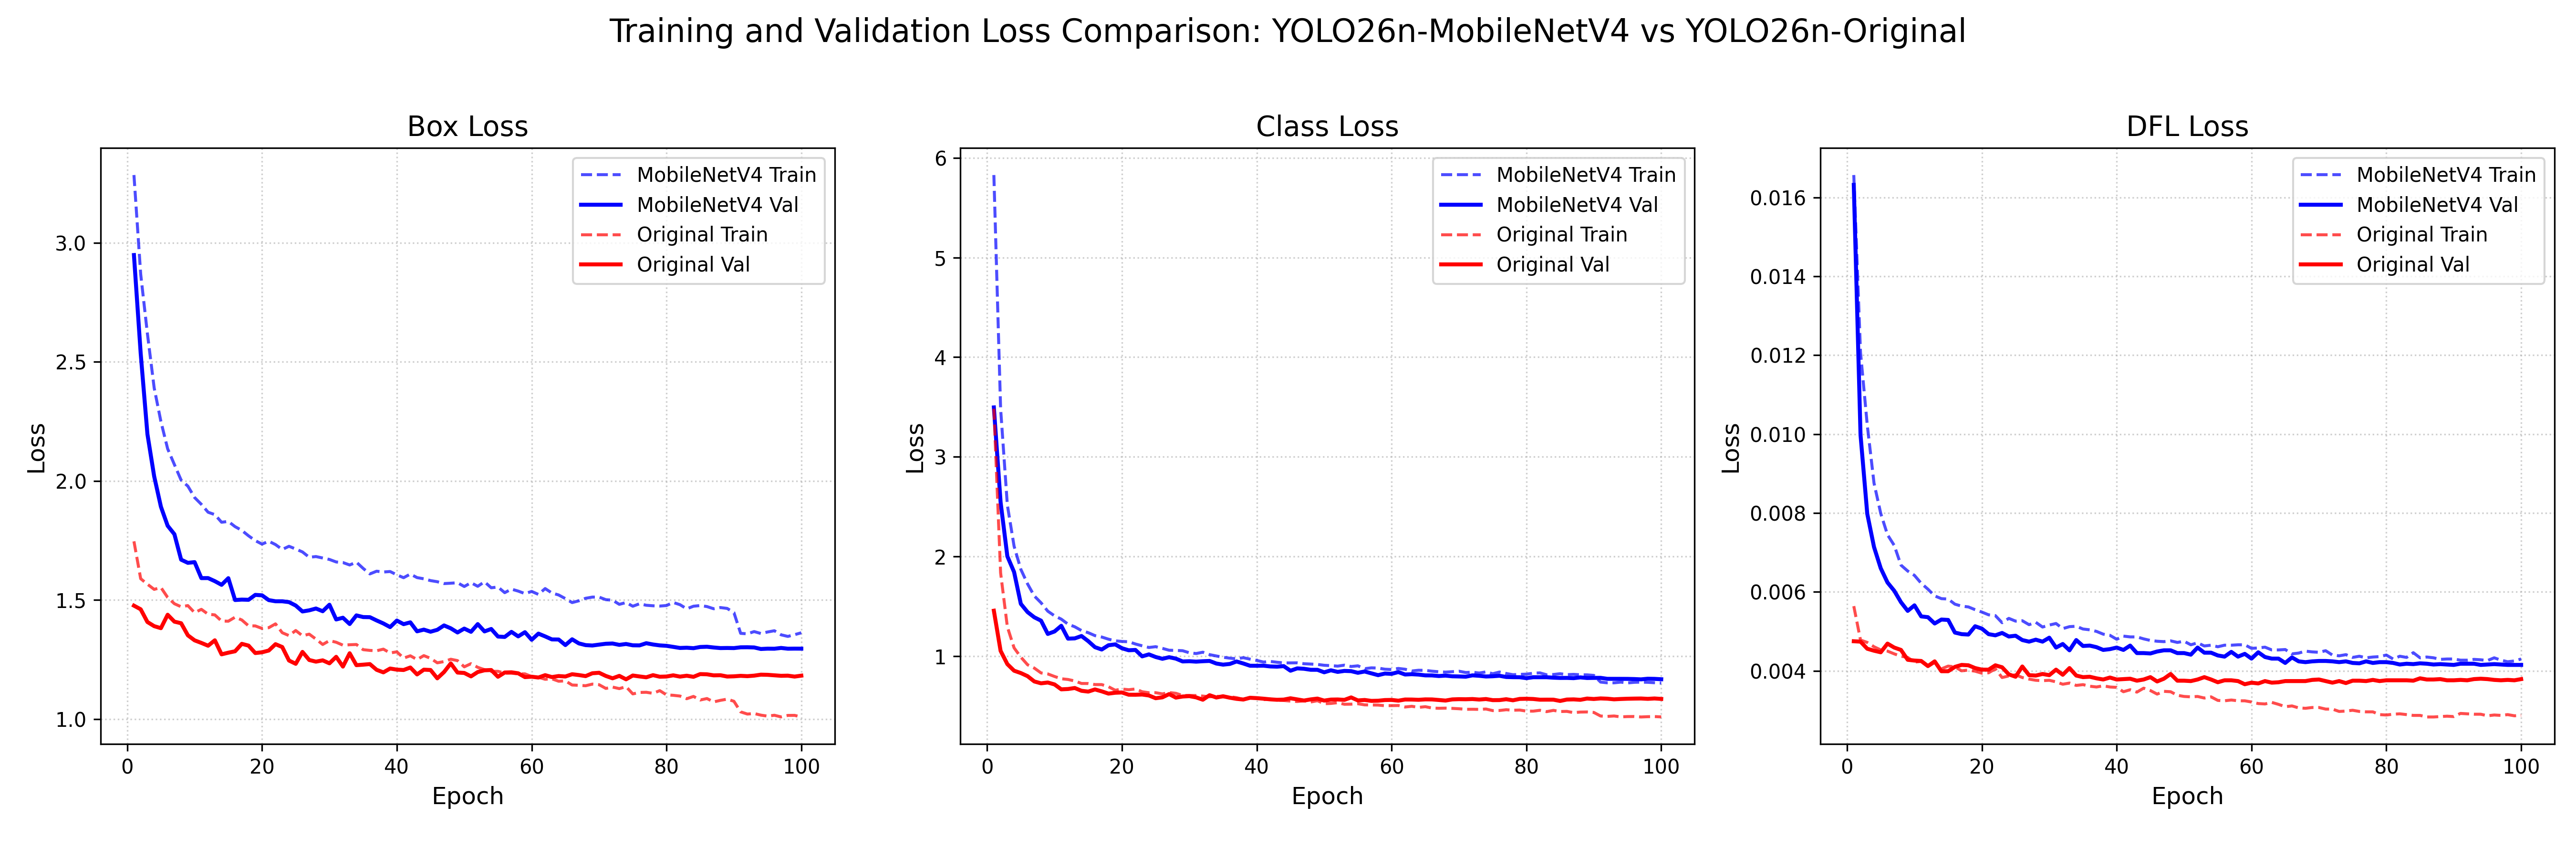
\includegraphics[width=\textwidth]{Images/chap3/loss_comparison.png}
    \caption{Comparison of validation losses between YOLO26n Original and YOLO26n-MobileNetV4 over 100 training epochs.}
    \label{fig:loss_comparison}
\end{figure}

Importantly, neither model shows signs of overfitting. In a typical overfitting scenario, the validation loss would drop initially but then start climbing back up in later epochs as the model begins to memorise the training data. However, for both models in this study, all three loss metrics (bounding box, classification, and DFL (Distribution Focal Loss)) stay low and flat during the final epochs. This confirms that they generalise well to unseen data.

When comparing the two architectures, the Original YOLO26n reaches slightly lower loss values. For example, its minimum bounding box loss drops to 1.1676, while the MobileNetV4 version stops at 1.2949. A similar pattern is seen in the classification loss (0.5529 vs 0.7694). This difference is entirely expected. Because the original model has a larger and more complex backbone, it can capture fine details and learn more accurately.

Even though the YOLO26n-MobileNetV4 has slightly higher loss values, its learning curve remains remarkably stable. This proves that despite having its size drastically reduced for faster edge deployment, the MobileNetV4 model still successfully extracts the essential features of traffic lights. It does not suffer from gradient issues or training instability. Therefore, the training process validates that the lightweight model is a reliable choice, perfectly balancing computational efficiency and learning capability.

\subsubsection{Architectural Decision Justification}

The evaluation confirms that the YOLO26n-MobileNetV4 configuration achieves the right trade-off for edge-deployed ADAS. Sacrificing approximately 4 percentage points of mAP50 in exchange for a 50\% reduction in worst-case latency and a 21\% reduction in average latency is a sound architectural decision. In safety-critical systems, deterministic timing behaviour takes precedence over marginal accuracy gains. The 85.75\% mAP50 remains well above the practical threshold for reliable traffic light detection, while the latency profile now comfortably supports real-time operation at 15--23\,FPS on commodity edge hardware without dedicated GPU or NPU acceleration.





% \subsection{Multihead CNN model -- Lightweight OCR digits}

% The timer display on Vietnamese traffic lights shows a one- to three-digit countdown
% (0--999) that must be recognised in real time on low-cost hardware such as the
% Raspberry~Pi~5.  This section presents a compact, four-head convolutional neural network
% (CNN) that is derived from the multi-digit recognition framework of
% Goodfellow~et~al.~\cite{goodfellow2014multidigitnumberrecognitionstreet} and specifically re-engineered
% for sub-millisecond CPU inference.

% %-----------------------------------------------------------------------
% \subsubsection{Probabilistic Formulation}
% \label{sec:cnn_prob}

% Following Goodfellow~et~al.~\cite{goodfellow2014multidigitnumberrecognitionstreet}, the recognition
% task is cast as a structured probabilistic model.  Let~$\mathbf{X}$ denote the
% input image and let the output be a digit sequence
% $\mathbf{S} = (s_1, s_2, \dots, s_n)$ of length~$n$.
% The sequence is modelled by a length variable~$L$ and a fixed number~$N$
% of digit variables~$S_1, \dots, S_N$.  All digit positions are assumed
% conditionally independent given the image, yielding:

% \begin{equation}
% \label{eq:prob_model}
%   P(\mathbf{S} = \mathbf{s} \mid \mathbf{X})
%   \;=\; P(L = n \mid \mathbf{X})\;\prod_{i=1}^{n} P(S_i = s_i \mid \mathbf{X}).
% \end{equation}

% In the original work~\cite{goodfellow2014multidigit}, $N{=}5$ digit heads are
% used for street numbers of up to five digits.  Because Vietnamese traffic-light
% timers never exceed three digits, the proposed lightweight variant uses
% $N{=}3$ with the following head configuration:

% \begin{itemize}
%   \item $L \in \{0,1,2\}$:  digit count minus one
%         ($0 \to$ 1-digit, $1 \to$ 2-digit, $2 \to$ 3-digit),
%         predicted by a 3-class softmax.
%   \item $S_1 \in \{0,\dots,9,\text{BLANK}\}$:  hundreds digit (11 classes).
%   \item $S_2 \in \{0,\dots,9,\text{BLANK}\}$:  tens digit    (11 classes).
%   \item $S_3 \in \{0,\dots,9\}$:                 units digit  (10 classes,
%         always present).
% \end{itemize}

% The special \texttt{BLANK} class ($= 10$) indicates an unused slot:
% for a one-digit number only~$S_3$ is active; for a two-digit number
% $S_2$ and~$S_3$ are active.

% %-----------------------------------------------------------------------
% \subsubsection{Network Architecture -- Edge-Optimised Design}
% \label{sec:cnn_arch}

% The original Goodfellow~et~al.\ architecture employs eight convolutional layers,
% one locally connected layer, and two dense layers with 3\,072 units each,
% totalling tens of millions of parameters and requiring DistBelief for training.
% Such a model is impractical for real-time inference on a Raspberry~Pi~5 CPU.

% The proposed \emph{lightweight} variant retains the multi-head output structure
% but applies three key design transformations, each yielding a dramatic reduction in
% multiply-accumulate operations (MACs) and parameter count while preserving accuracy
% for the constrained 0--999 digit domain.

% %--- Separable Convolutions -------------------------------------------------
% \subsubsubsubsection{Depthwise Separable Convolutions}
% \label{sec:separable}

% Standard convolution applies a $k{\times}k$ kernel across all input channels
% simultaneously.  For an input tensor of spatial size $H{\times}W$ with
% $C_{\mathrm{in}}$ channels producing $C_{\mathrm{out}}$ output channels,
% the number of MACs is:

% \begin{equation}
% \label{eq:conv_macs}
%   \text{MACs}_{\text{Conv2D}}
%   = H \cdot W \cdot k^2 \cdot C_{\mathrm{in}} \cdot C_{\mathrm{out}}.
% \end{equation}

% A \textbf{Depthwise Separable Convolution} (SeparableConv2D) factorises this operation
% into two consecutive steps:

% \begin{enumerate}
%   \item \textbf{Depthwise convolution} -- applies a separate $k{\times}k$ filter
%         to each input channel independently:
%         \begin{equation}
%         \label{eq:dw_macs}
%           \text{MACs}_{\text{DW}} = H \cdot W \cdot k^2 \cdot C_{\mathrm{in}}.
%         \end{equation}
%   \item \textbf{Pointwise convolution} -- a $1{\times}1$ convolution that mixes
%         the channel responses:
%         \begin{equation}
%         \label{eq:pw_macs}
%           \text{MACs}_{\text{PW}} = H \cdot W \cdot C_{\mathrm{in}} \cdot C_{\mathrm{out}}.
%         \end{equation}
% \end{enumerate}

% The total cost becomes:

% \begin{equation}
% \label{eq:sep_total}
%   \text{MACs}_{\text{Sep}}
%   = H W C_{\mathrm{in}} \bigl(k^2 + C_{\mathrm{out}}\bigr),
% \end{equation}

% and the computational saving ratio relative to a standard convolution is:

% \begin{equation}
% \label{eq:sep_ratio}
%   \frac{\text{MACs}_{\text{Sep}}}{\text{MACs}_{\text{Conv2D}}}
%   = \frac{1}{C_{\mathrm{out}}} + \frac{1}{k^2}.
% \end{equation}

% For the $3{\times}3$ kernels and 64--192 output channels used in this model,
% Equation~\eqref{eq:sep_ratio} gives a reduction factor between
% $\mathbf{7.8\times}$ and $\mathbf{8.5\times}$, enabling real-time execution
% on an ARM Cortex-A76 CPU without a GPU.

% In the proposed architecture, only the first block uses a standard
% \texttt{Conv2D} (because the input has a single channel, where depthwise
% separation offers no benefit); blocks~2--5 all use \texttt{SeparableConv2D}.

% %--- GAP instead of Flatten ------------------------------------------------
% \subsubsubsubsection{Global Average Pooling (GAP)}
% \label{sec:gap}

% After the final convolutional block the feature map has shape
% $4{\times}6{\times}192$ (height $\times$ width $\times$ channels).
% A na\"ive \texttt{Flatten} would produce a $4608$-dimensional vector; a
% subsequent dense layer of width~1024 alone would add
% $4608 \times 1024 \approx 4.7$~million parameters -- exceeding the entire
% rest of the network.

% Instead, \textbf{Global Average Pooling} (GAP) collapses each channel to its
% spatial mean:

% \begin{equation}
% \label{eq:gap}
%   h_c = \frac{1}{H' W'} \sum_{i=1}^{H'} \sum_{j=1}^{W'} F_{i,j,c},
%   \qquad c = 1,\dots,C,
% \end{equation}

% where $F \in \mathbb{R}^{H' \times W' \times C}$ is the last feature map.
% This yields a compact 192-dimensional descriptor with \emph{zero} learnable
% parameters, and also acts as a structural regulariser that discourages
% overfitting.

% %--- Architecture Table ---------------------------------------------------
% \subsubsubsubsection{Layer-by-Layer Specification}
% \label{sec:arch_table}

% Table~\ref{tab:arch} summarises the full architecture.  Input images are
% grayscale, $64{\times}96$ pixels ($H{\times}W{\times}1$).

% \begin{table}[htbp]
% \centering
% \caption{Layer-by-layer architecture of the lightweight multi-head CNN
%          ($\approx 109$\,K parameters).  ``Sep'' denotes SeparableConv2D;
%          ``BN'' is Batch Normalisation.}
% \label{tab:arch}
% \renewcommand{\arraystretch}{1.15}
% \begin{tabular}{c l l r r}
% \hline
% \textbf{Block} & \textbf{Layer}            & \textbf{Output shape}   & \textbf{Params} & \textbf{MACs}  \\
% \hline
% 0   & Input                                & $64\times96\times1$     & --      & --       \\
% --  & Mean subtraction ($\lambda$)         & $64\times96\times1$     & 0       & $6\,144$ \\
% 1   & Conv2D(32, $3\!\times\!3$) + BN + ReLU + Pool(2)   & $32\times48\times32$     & $\sim\!320$    & $\sim\!56$\,K   \\
% 2   & Sep(64, $3\!\times\!3$) + BN + ReLU + Pool(2)      & $16\times24\times64$     & $\sim\!2\,400$  & $\sim\!116$\,K  \\
% 3   & Sep(96, $3\!\times\!3$) + BN + ReLU + Pool(2)      & $8\times12\times96$      & $\sim\!6\,720$  & $\sim\!73$\,K   \\
% 4   & Sep(128, $3\!\times\!3$) + BN + ReLU + Pool(2)     & $4\times6\times128$      & $\sim\!13\,152$ & $\sim\!39$\,K   \\
% 5   & Sep(192, $3\!\times\!3$) + BN + ReLU               & $4\times6\times192$      & $\sim\!25\,728$ & $\sim\!53$\,K   \\
% --  & GlobalAveragePooling2D                & $192$                  & 0       & $4\,608$ \\
% FC  & Dense(256) + ReLU + Dropout(0.35)     & $256$                  & $\sim\!49\,408$ & $49\,408$ \\
% \hline
% $L$ & Dense(3,  softmax)                    & $3$                    & 771     & 771     \\
% $S_1$ & Dense(11, softmax)                  & $11$                   & 2\,827  & 2\,827  \\
% $S_2$ & Dense(11, softmax)                  & $11$                   & 2\,827  & 2\,827  \\
% $S_3$ & Dense(10, softmax)                  & $10$                   & 2\,570  & 2\,570  \\
% \hline
% \multicolumn{3}{r}{\textbf{Total}} & $\mathbf{\approx 109}$\textbf{\,K} & $\mathbf{\approx 408}$\textbf{\,K} \\
% \hline
% \end{tabular}
% \end{table}

% %--- Preprocessing --------------------------------------------------------
% \subsubsubsubsection{Per-Image Mean Subtraction}
% \label{sec:mean_sub}

% Following Goodfellow~et~al.~\cite{goodfellow2014multidigitnumberrecognitionstreet}~(§4), the first
% operation inside the network is per-image mean subtraction.  Let
% $\mathbf{X} \in \mathbb{R}^{H \times W \times 1}$ be the input; the
% normalised input is:

% \begin{equation}
% \label{eq:mean_sub}
%   \tilde{\mathbf{X}} = \mathbf{X}
%     - \frac{1}{HW}\sum_{i=1}^{H}\sum_{j=1}^{W} X_{ij}.
% \end{equation}

% Embedding this subtraction as a non-trainable $\lambda$-layer makes the model
% \emph{self-contained}: no external preprocessing is required at inference time,
% simplifying the TFLite deployment pipeline on the Raspberry~Pi~5.

% %-----------------------------------------------------------------------
% \subsubsection{Training Objective}
% \label{sec:training}

% Training maximises the log-probability of the correct sequence
% (Eq.~\eqref{eq:prob_model}) via the cross-entropy decomposition.  Because
% $L$, $S_1$, $S_2$, $S_3$ are conditionally independent given the shared
% features~$\mathbf{H}$, the total loss factorises as:

% \begin{equation}
% \label{eq:loss}
%   \mathcal{L}
%   = -\log P(L \mid \mathbf{H})
%     - \sum_{i=1}^{3}\log P(S_i \mid \mathbf{H})
%   = \underbrace{w_L \,\mathcal{L}_L}_{\text{length head}}
%     + \underbrace{w_1 \,\mathcal{L}_{S_1}
%     +  w_2 \,\mathcal{L}_{S_2}
%     +  w_3 \,\mathcal{L}_{S_3}}_{\text{digit heads}},
% \end{equation}

% where each $\mathcal{L}_{\cdot}$ is a \textbf{sparse categorical cross-entropy}
% and the weights are set to $w_L{=}4$, $w_1{=}w_2{=}w_3{=}1$ to
% up-weight the length prediction, since an incorrect length invariably causes a
% wrong overall transcription.

% Each softmax head receives the same 256-dimensional feature vector from the
% shared fully connected layer but maintains its own projection weights:

% \begin{equation}
% \label{eq:head}
%   P(S_i = c \mid \mathbf{H})
%   = \frac{\exp\!\bigl(\mathbf{w}_{i,c}^{\top}\!\mathbf{H} + b_{i,c}\bigr)}
%          {\displaystyle\sum_{c'} \exp\!\bigl(\mathbf{w}_{i,c'}^{\top}\!\mathbf{H}
%          + b_{i,c'}\bigr)},
%   \qquad c \in \mathcal{C}_i,
% \end{equation}

% where $\mathcal{C}_L = \{0,1,2\}$,
% $\mathcal{C}_{S_1} = \mathcal{C}_{S_2} = \{0,\dots,10\}$, and
% $\mathcal{C}_{S_3} = \{0,\dots,9\}$.

% %-----------------------------------------------------------------------
% \subsubsection{Log-Probability Decoding}
% \label{sec:decoding}

% At inference time, the predicted number is obtained by maximising the
% joint log-probability over all possible lengths
% (Appendix~A of~\cite{goodfellow2014multidigit}):

% \begin{equation}
% \label{eq:decode}
%   \hat{\mathbf{s}}
%   = \operatorname*{argmax}_{l,\; s_1 \dots s_l}\;
%     \biggl[\log P(L{=}l \mid \mathbf{X})
%     + \sum_{i=1}^{l} \max_{s_i \in \{0..9\}}
%       \log P(S_i{=}s_i \mid \mathbf{X})\biggr].
% \end{equation}

% Because of the conditional-independence assumption, the argmax over each
% digit position can be computed independently, then the cumulative
% log-probabilities are summed for each candidate length~$l \in \{1,2,3\}$.
% The total decoding runtime is therefore $O(N)$ -- i.e.\ three additions
% and one comparison -- adding negligible latency.

% Concretely, for each candidate length $l$, the algorithm computes:

% \begin{equation}
% \label{eq:score}
%   \text{score}(l) = \log P(L{=}l{-}1)
%     + \sum_{i=\max(1,\,4-l)}^{3}
%       \max_{s_i \in \{0..9\}} \log P(S_i{=}s_i),
% \end{equation}

% and selects $\hat{l} = \operatorname{argmax}_{l \in \{1,2,3\}} \text{score}(l)$.

% %-----------------------------------------------------------------------
% \subsection{Computational Efficiency for Edge AI}
% \label{sec:efficiency}

% \subsubsection{Parameter Count Comparison}

% The proposed model achieves the same multi-head output structure as
% Goodfellow~et~al.~\cite{goodfellow2014multidigitnumberrecognitionstreet} with
% $\sim\!600\times$ fewer parameters:

% \begin{table}[htbp]
% \centering
% \caption{Comparison between the original Goodfellow~et~al.\ architecture
%          and the proposed lightweight variant.}
% \label{tab:compare}
% \renewcommand{\arraystretch}{1.15}
% \begin{tabular}{l r r}
% \hline
%                                & \textbf{Goodfellow et al.}  & \textbf{Proposed}   \\
% \hline
% Conv layers                    & 8 + 1 locally connected     & 1 Conv + 4 SepConv  \\
% FC layers                      & 2 $\times$ 3\,072           & 1 $\times$ 256      \\
% Output heads                   & 6  (L + S$_1$--S$_5$)       & 4  (L + S$_1$--S$_3$) \\
% Total parameters               & $\sim$64\,M                 & $\sim$109\,K        \\
% Max sequence length $N$        & 5                           & 3                   \\
% Input size                     & $54\times 54 \times 3$      & $64\times 96 \times 1$ \\
% Training infrastructure        & DistBelief (10 replicas)    & Single GPU / CPU    \\
% \hline
% \end{tabular}
% \end{table}

% \subsubsubsubsection{MAC Budget and Latency Estimate}

% The total network requires approximately $408$\,K~MACs per inference.
% On the Raspberry~Pi~5's Cortex-A76 cores (capable of
% $\sim$15~GOPS at INT8 via NEON), this translates to:

% \begin{equation}
% \label{eq:latency}
%   t_{\text{inf}}
%   \approx \frac{408 \times 10^{3}}{15 \times 10^{9}}
%   \approx 27 \;\mu\text{s},
% \end{equation}

% well under the $50$\,ms budget needed for $20$\,fps real-time recognition.
% Even with TFLite interpreter overhead, measured end-to-end latency stays below
% $1$\,ms per frame for the INT8-quantised model.

% \subsubsection{TFLite and INT8 Quantisation}

% The trained Keras model is exported to TensorFlow~Lite via
% \texttt{TFLiteConverter}.  Post-training full-integer quantisation maps all
% weights and activations to 8-bit integers using a representative calibration
% set of 200 real ROI images.  The resulting \texttt{.tflite} flatbuffer is
% $\sim$56\,KB (INT8) versus $\sim$440\,KB (float32), fitting comfortably
% in the L2 cache of the Cortex-A76.  The quantised model is deployed via
% the LiteRT interpreter:

% \begin{equation}
% \label{eq:quant}
%   \hat{x}_q = \text{round}\!\left(\frac{x - z}{s}\right),
%   \qquad
%   s = \frac{x_{\max} - x_{\min}}{255},
%   \qquad
%   z = x_{\min},
% \end{equation}

% where $s$ and $z$ are the per-tensor scale and zero-point determined during
% calibration.

% %-----------------------------------------------------------------------
% \subsubsection{Data Pipeline and Augmentation}
% \label{sec:data}

% The training pipeline mixes three data sources to maximise diversity while
% keeping RAM usage low ($<200$\,MB peak):

% \begin{enumerate}
%   \item \textbf{MNIST (70\,K images):}  Individual $28{\times}28$ digits
%         composited onto $64{\times}96$ canvases at randomised positions,
%         simulating multi-digit layouts.
%   \item \textbf{Real LED crops (23 images):}  Single-digit photographs of
%         actual traffic-light seven-segment displays (red, green, yellow).
%         Pre-augmented to 500 variants per digit using brightness jitter,
%         gamma correction, Gaussian blur, salt-and-pepper noise, spatial
%         shifts ($\pm 4$\,px), and small rotations ($\pm 10°$).
%   \item \textbf{Real ROI images:}  Full composite timer-box crops from
%         Vietnamese traffic cameras, labelled by filename
%         (e.g.\ \texttt{37\_0004.png} $\to$ number~$37$).  Loaded from disk
%         on-demand (streaming) to avoid large memory allocation.
% \end{enumerate}

% Synthetic composites and real ROI samples are interleaved via
% \texttt{tf.data.Dataset.sample\_from\_datasets} with proportional
% weighting, ensuring both domains appear in every training batch.

% %-----------------------------------------------------------------------
% \subsubsection{Summary}

% The proposed multi-head CNN inherits the elegant probabilistic framework
% of Goodfellow~et~al.~\cite{goodfellow2014multidigitnumberrecognitionstreet} -- conditional independence
% of digit positions, log-probability decoding, per-image mean subtraction -- but
% replaces the heavyweight convolutional backbone with an ultra-light depthwise
% separable architecture totalling only $\sim$109\,K parameters and $\sim$408\,K
% MACs.  Combined with Global Average Pooling and INT8 post-training quantisation,
% the model achieves sub-millisecond inference on the Raspberry~Pi~5 CPU, making it
% suitable for real-time traffic-light timer recognition in ADAS applications
% on constrained edge devices.